\documentclass[12pt]{report}

%-------------------- Packages ---------------------%
\usepackage{lmodern}           % Load lmodern font
\usepackage[french]{babel}     % French language support
\usepackage[utf8]{inputenc}    % UTF-8 encoding
\usepackage[T1]{fontenc}       % Output font encoding
\usepackage{tikz}

\usetikzlibrary{shapes,arrows,positioning,fit}
\usepackage[top=2cm,bottom=2.5cm,right=2cm,left=2cm]{geometry} % Initial Page margins
\usepackage{quoting}           % For quoting environment
\usepackage{graphicx}          % For including graphics
\usepackage{hyperref}          % For hyperlinks
\usepackage{changepage}        % For adjusting page margins
\usepackage{subcaption}        % For sub-captions
\usepackage[footnote]{acronym} % For acronyms
\usepackage{blindtext}         % For dummy text
\usepackage[dvipsnames]{xcolor}% For color
\usepackage{amsmath,amsfonts,amssymb} % For math symbols and fonts
\usepackage{makeidx}           % For indexing
\usepackage{colortbl}          % For colored tables
\usepackage{float}             % For floating objects
\usepackage{wrapfig}           % For wrapped figures
\usepackage{placeins}          % For keeping floats in sections
\usepackage{titlesec}          % For customizing section titles
\usepackage{fancyhdr}          % For headers and footers
\usepackage{afterpage}         % For changing the geometry on specific pages
\usepackage{underscore}
\usepackage[backend=bibtex]{biblatex} % For bibliography
\usepackage[page,toc,titletoc,title]{appendix} % For appendices
\usepackage{pdfpages}
\usepackage{hyperref}          % For hyperlinks

%-------------------- Color Definitions ---------------------%
\definecolor{orangecustom}{RGB}{230,115,0}

%-------------------- Customizations ---------------------%
% Footnote size
\renewcommand{\footnotesize}{\fontsize{7pt}{9pt}\selectfont}

% Table of contents and section numbering depth
\setcounter{tocdepth}{3}
\setcounter{secnumdepth}{3}

% Table and figure captions
\renewcommand{\tablename}{Tableau}
\renewcommand{\figurename}{Figure}

% Chapter title format and spacing
\titleformat{\chapter}[display]
{\normalfont\huge\bfseries}{\chaptername\ \thechapter}{20pt}{\Huge}
\titlespacing*{\chapter}{0pt}{-20pt}{40pt}

% Custom chapter opening page with quote
\newcommand{\mychapter}[2]{%
	\clearpage
	\refstepcounter{chapter}%
	\addcontentsline{toc}{chapter}{\Roman{chapter}. #1}%
	\markboth{#1}{#1}%
	\thispagestyle{plain}%
	\vspace*{0.2\textheight}
	\begin{center}
		\begin{minipage}{0.9\textwidth}
			\centering
			{\large\bfseries CHAPTER \Roman{chapter}\par}
			\vspace{0.5cm}
			{\Huge\bfseries #1\par}
			\vspace{1.5cm}
			{\linespread{1.6}\selectfont\Large\itshape #2\par}
		\end{minipage}
	\end{center}
	\vspace*{\fill}
	\clearpage
	\pagestyle{fancy}%
}

% Round (circular) cropped picture, uniform size, for team photos
\newcommand{\roundpic}[1]{%
	\begin{tikzpicture}[baseline=(c.base)]
		\node[circle, minimum size=2.8cm, inner sep=0pt] (c) {};
		\begin{scope}
			\clip (c.center) circle (1.4cm);
			\node at (c.center) {\includegraphics[width=2.8cm,height=2.8cm]{#1}};
		\end{scope}
		\draw[line width=1pt, gray!60] (c.center) circle (1.4cm);
	\end{tikzpicture}%
}

% French language customizations for appendices
\addto\captionsfrench{%
	\renewcommand\appendixname{Annexe}
	\renewcommand\appendixpagename{Annexes}
	\renewcommand{\appendixtocname}{Annexes}
}

%-------------------- Page Style ---------------------%
\pagestyle{fancy}
\fancyhf{} % Clear all header and footer fields
\fancyhead[L]{\leftmark} % Chapter title in the left header
\fancyfoot[C]{\thepage} % Page number in the right header
\renewcommand{\headrulewidth}{0.4pt} % Line thickness for the header
\setlength{\headheight}{14.5pt}

%-------------------- Document Start ---------------------%
\begin{document}
	
	% Title page
	\pagestyle{empty} % Remove page number from title page

        % ---------Page De Garde---------%
	\definecolor{orangecustom}{RGB}{230,115,0}
\definecolor{bluecustom}{RGB}{0,51,102}

\begin{figure}[t]
    \centering
    
\includegraphics[width=1\textwidth]{LOGOS/Screenshot 2024-08-22 214355.png}
\end{figure}

\vspace{1.5cm}

\begin{center}
 {\Large\bfseries\textbf{DÉPARTEMENT MATHÉMATIQUES ET INFORMATIQUE}}

    \vspace{1cm}

    {\large\bfseries Filière :}\\
    \vspace{0.5cm}
     {\color{bluecustom}\large\bfseries «Ingénierie Informatique: Big Data et Cloud Computing»}

    \vspace{0.6cm}

    {\color{black}\Huge\bfseries\textbf{Rapport du\\[0.2cm] Projet de fin d'etude}}
    \vspace{1cm}

    \begin{tikzpicture}
        % Define the rectangle with the text
        \node[draw=orangecustom, rectangle, line width=2pt, inner sep=20pt, text width=0.7\textwidth, align=center] (box) {
            \color{black}\Huge{Projet d'innovation : Job-Ai  }
        };

        % Draw two lines inside the rectangle
        \draw[orangecustom, thick] (box.south west) -- (box.south east); % Bottom line
        \draw[orangecustom, thick] (box.north west) -- (box.north east); % Top line
    \end{tikzpicture}

    \vspace{1.4cm}

    \begin{tikzpicture}
        % Define the rectangle with the text
        \node[draw=orangecustom, rectangle, line width=2pt, inner sep=20pt, text width=0.8\textwidth, align=center] (box) {
            \begin{minipage}{0.45\textwidth}
                \textbf{Réalisé par:}\\
                    - EL BADRY Mohammed\\
            \end{minipage}
            \hfill
            \begin{minipage}{0.45\textwidth}
                \textbf{Encadré par:}\\
                       - Othmane KINANE\\
                       - Pr. BOUSSELHAM Abdelmajid\\
            \end{minipage}
        };

        % Draw two lines inside the rectangle
        \draw[orangecustom, thick] (box.south west) -- (box.south east); % Bottom line
        \draw[orangecustom, thick] (box.north west) -- (box.north east); % Top line
    \end{tikzpicture}

    \vfill

    {\large\bfseries Année Universitaire: 2025-2026}
\end{center}

\vfill

% Footer
\begin{figure}[b]
    \centering
    
\includegraphics[width=1\textwidth]{LOGOS/Screenshot 2024-08-22 214411.png}
\end{figure}
	
	% Adjust margins for the rest of the document
	\newgeometry{top=2.5cm, bottom=2.5cm, right=2cm, left=2.5cm}
	\newpage
	
	% Preliminary pages with Roman numerals

	\pagenumbering{gobble}	% Remove the entire counter

	% Dedication
	% Adding an empty page
\newpage
\thispagestyle{empty}
\mbox{} % Empty page with no content

\chapter*{Dedication}
\addcontentsline{toc}{section}{\textbf{Dedication}}

\vspace{1.5cm}

\begin{center}
\itshape\large

To my dear parents,\\
whose unconditional love, patience, and sacrifices
have lighted every step of my journey.
Nothing I achieve would have been possible without you.

\vspace{1cm}

To my family,\\
for their constant encouragement and unwavering support.

\vspace{1cm}

To my teachers and mentors,\\
who shared their knowledge with generosity
and shaped the engineer I am becoming.

\vspace{1cm}

To my friends and colleagues,\\
for the moments of doubt we overcame together
and the joys we shared along the way.

\vspace{1cm}

To everyone who believed in me.

\vspace{2cm}

\upshape\normalsize\bfseries Mohammed El Badry

\end{center}


	\thispagestyle{plain}

	% Acknowledgment
	\chapter*{Acknowledgment}
\addcontentsline{toc}{section}{\textbf{Acknowledgment}}

\vspace{0.5cm}

Before presenting the work carried out during this end-of-study internship, I would like to express my sincere gratitude to all the people who contributed, directly or indirectly, to the success of this project.

\vspace{0.3cm}

I would first like to thank \textbf{Theodo Morocco} for the trust it placed in me by welcoming me within its teams. This internship gave me the opportunity to grow in a stimulating, demanding, and deeply human professional environment.

\vspace{0.3cm}

I extend my warmest thanks to my company supervisor, \textbf{Mr. Othmane Kinane}, for his guidance, his availability, and the quality of the feedback he provided throughout this experience. My gratitude also goes to \textbf{Yassine Ghazouan}, Tech Lead, and \textbf{Hamza Berraho}, Project Manager, whose technical insight and clear vision constantly steered the project in the right direction. I am also sincerely grateful to my coach, \textbf{Abdelaziz Afriad}, for his guidance and his mentorship throughout this journey, and for helping me become more integrated into this new environment.

\vspace{0.3cm}

I am equally grateful to my teammates, \textbf{Mohammed Bourhym} and \textbf{Ismail Drissi}, for their collaboration, their generosity in sharing knowledge, and the team spirit that made every challenge easier to overcome.

\vspace{0.3cm}

I would also like to express my deep appreciation to my academic supervisor, \textbf{Pr. Abdelmajid Bousselham}, for his attentive follow-up, his valuable advice, and his rigor, which greatly contributed to the quality of this report.

\vspace{0.3cm}

Finally, I address my thanks to the entire teaching staff of the \textbf{Department of Mathematics and Computer Science}, as well as to all those who, through their support and encouragement, accompanied me throughout these years of study.

\clearpage

	\thispagestyle{plain}

	% Abstract
	\chapter*{Abstract}
\addcontentsline{toc}{section}{\textbf{Abstract}}

\vspace{0.5cm}

Mobile applications built by software consultancies such as \textbf{Theodo} must comply with the publication rules of the \textbf{Apple App Store and Google Play.} In practice, non-compliance is often discovered only at the very end of the development cycle, when the application is submitted to the stores. A late rejection then causes costly \textbf{rework and delivery delays} for applications already in production. This work, carried out as part of the \textbf{Mobile Software Factory} project, addresses this problem by shifting compliance verification to the left, that is, earlier and continuously throughout development.

\vspace{0.3cm}

The proposed solution is an \textbf{automated compliance audit tool}, delivered as a structured \textit{skill} executed by an AI coding agent. Rather than a classic static analyzer, it relies on auditable policy packs that the agent applies through reasoning, following a five-step workflow: framework detection, review-oriented codebase understanding, business-domain selection, application of the relevant policies, and report generation. The approach is deliberately scope-aware, evaluating only the guidelines relevant to the features the application actually uses, and evidence-based, so that every finding is traced both to an observed code path and to a written policy rule.

\vspace{0.3cm}

Because the tool is driven by a language model, its output cannot be validated with classical unit tests. A behavioral evaluation suite was therefore built with \textbf{Promptfoo}, combining minimal fixture projects, paired compliant/non-compliant scenarios, \textbf{deterministic assertions, and rubric-based judgments} to guarantee that the audit identifies the right issues, cites the right evidence, and avoids hallucinated findings.

\vspace{0.8cm}

\noindent\textbf{Keywords:} Store compliance, Mobile applications, App Store, Google Play, Shift-left, AI agent, LLM, Skill, Permissions, Promptfoo, Proof of concept.

\clearpage

	\thispagestyle{plain}

	% Résumé
	\chapter*{Résumé}
\addcontentsline{toc}{section}{\textbf{Résumé}}

\vspace{0.5cm}

Les applications mobiles développées par des cabinets de conseil tels que \textbf{Theodo} doivent respecter les règles de publication de l'\textbf{Apple App Store et de Google Play.} En pratique, la non-conformité n'est souvent détectée qu'à la toute fin du cycle de développement, au moment de la soumission de l'application sur les stores. Un rejet tardif entraîne alors, à grands frais, des \textbf{reprises et des retards de livraison} pour les applications déjà en production. Ce travail, réalisé dans le cadre du projet \textbf{Mobile Software Factory}, répond à cette problématique en déplaçant la vérification de conformité « vers la gauche », c'est-à-dire plus tôt et de manière continue tout au long du développement.

\vspace{0.3cm}

La solution proposée est un \textbf{outil d'audit de conformité automatisé}, livré sous la forme d'une \textit{skill} structurée et exécutée par un agent de programmation basé sur l'intelligence artificielle. Plutôt qu'un analyseur statique classique, il s'appuie sur des paquets de règles auditables que l'agent applique par raisonnement, en suivant un processus en cinq étapes : détection du framework, compréhension du code orientée revue, sélection du domaine métier, application des règles pertinentes et génération du rapport. L'approche est volontairement ciblée, n'évaluant que les directives pertinentes pour les fonctionnalités réellement utilisées par l'application, et fondée sur des preuves, de sorte que chaque constat est rattaché à la fois à un comportement observé dans le code et à une règle écrite.

\vspace{0.3cm}

Comme l'outil est piloté par un modèle de langage, sa sortie ne peut être validée par des tests unitaires classiques. Une suite d'évaluation comportementale a donc été construite avec \textbf{Promptfoo}, combinant des projets de test minimaux, des scénarios appariés conformes / non conformes, \textbf{des assertions déterministes et des jugements basés sur des grilles d'évaluation} afin de garantir que l'audit identifie les bons problèmes, cite les bonnes preuves et évite les constats hallucinés.

\vspace{0.8cm}

\noindent\textbf{Mots-clés :} Conformité aux stores, Applications mobiles, App Store, Google Play, Shift-left, Agent IA, LLM, Skill, Permissions, Promptfoo, Preuve de concept.

\clearpage

	\thispagestyle{plain}

	% Table of Contents
	\tableofcontents
	\clearpage
	
	% List of Figures
	\listoffigures
	\clearpage
	
	% Main Content with Arabic numerals
	\pagenumbering{arabic}
	\setcounter{page}{1}
	\pagestyle{fancy}
	% Include main content chapters
	\chapter*{\Huge General Introduction}
\addcontentsline{toc}{section}{\textbf{General Introduction}}

As the culmination of my pursuit of a state engineering diploma in Software Engineering, Big Data, and Cloud Computing, I undertook an end-of-study internship at \textbf{Theodo Morocco}, a digital consultancy firm recognized for delivering high-impact web and mobile software solutions for its clients. This internship offered the opportunity to confront a concrete industrial problem and to design, build, and evaluate a complete solution within a professional engineering environment.

\vspace{0.3cm}

A consultancy such as Theodo regularly builds mobile applications that must eventually be published on the Apple App Store and Google Play. Each store enforces a detailed set of review guidelines and developer policies, and any violation can lead to the rejection of an application. The recurring difficulty is that this verification happens too late: teams develop an application over several weeks or months, and the non-compliance is only discovered at submission time, at the worst possible moment, right before delivery. This \textit{late detection} causes costly rework and delays, while applications already in production accumulate a growing \textit{compliance debt} as store requirements evolve. The core insight behind this project is that compliance should be verified continuously, as the application is being built, rather than as a one-shot gate at the very end.

\vspace{0.3cm}

This work was carried out within the \textbf{Mobile Software Factory} project, a collaborative initiative at Theodo aimed at improving the reliability and the speed of mobile application delivery. The project brought together a cross-functional team composed of developers, a tech lead, and a project manager. My contribution focused on the store-compliance component, materialized as an automated audit tool that a developer can run as a command during development to obtain a clear and actionable compliance status of the application.

\vspace{0.3cm}

The solution is designed as a structured \textit{skill} executed by an AI coding agent. It inspects the source code and configuration of a cross-platform mobile application, applies a set of auditable policy rules, and produces a report describing what was checked, what passes, what fails, and how each issue should be remediated. The approach is deliberately scope-aware, evaluating only the guidelines relevant to the features the application actually uses, and evidence-based, so that each finding is justified by an observed behavior and a written rule rather than by guesswork. Particular attention was given to the quality assurance strategy, since a tool driven by a language model cannot be validated through classical unit testing and required a dedicated behavioral evaluation methodology.

\vspace{0.5cm}

This report is structured into several chapters to provide a clear and progressive overview of my contributions:

\vspace{0.3cm}

\noindent\textbf{Chapter I -- Host Organization \& Project Context} introduces Theodo Morocco and its place within the international Theodo Group, the work culture that framed the internship, the project team, and the overall mission. It situates the internship in its professional environment before any technical detail is discussed.

\vspace{0.2cm}

\noindent\textbf{Chapter II -- } 

\vspace{0.2cm}

\noindent\textbf{Chapter III -- } 

\vspace{0.2cm}

\noindent\textbf{Chapter IV -- }

\vspace{1cm}

	\renewcommand{\chaptername}{Chapitre}
\label{part:Analyse du Problème}
\chapter{Host Organization \& Project Context}

% Chapter 1
A concise overview of Theodo’s history, mission, core values, and culture, along with the thorough hiring and onboarding processes that shaped my internship experience

\section{Introduction}

This opening chapter establishes the comprehensive foundation for understanding both the organizational environment and project context that shaped my end-of-study internship experience. The chapter bridges the gap between the professional setting at Theodo Morocco and the specific challenges of modernizing the National Sports Federation's critical infrastructure, demonstrating how organizational culture and project requirements aligned to create an ideal learning environment.

The first section introduces Theodo Morocco, the dynamic software consultancy where I conducted my internship. From its origins as Nimbleways in 2017 to its integration into the international Theodo Group in 2019, the company has established itself as a key player in delivering high-quality digital solutions across North Africa. Theodo's core values—rigor, pragmatism, eagerness to progress, and team spirit—directly influenced how the FDME project was approached, executed, and delivered. Understanding these values is essential for appreciating the methodical yet agile approach that characterized every aspect of the project.

The second section presents the specific project context that brought together Theodo's expertise with the federation's urgent modernization needs. The National Sports Federation, representing one of Europe's most significant sporting institutions, manages over 500,000 licensed members across 2,300 clubs and orchestrates more than 70,000 matches annually. This massive operational scale demanded sophisticated digital infrastructure to maintain standards of fairness, transparency, and operational excellence throughout the national handball ecosystem.

The third section analyzes the legacy Electronic Match Sheet (FDME) system that had served as the backbone of match reporting for nearly fifteen years. Originally developed in the early 2010s with Windows desktop applications and limited web interfaces, the system had accumulated critical technical limitations including platform compatibility issues, connectivity resilience problems, user interface constraints, and performance degradation under load. These technical bottlenecks translated into tangible operational challenges affecting referees, coaches, administrators, and volunteers nationwide.

Together, these sections establish how Theodo's methodical approach to software delivery perfectly matched the federation's need for reliable, user-centered solutions capable of supporting distributed operations across thousands of venues with varying technical capabilities. The chapter demonstrates how organizational excellence and project complexity intersected to create an environment ideal for applying cutting-edge software engineering practices to challenges of national significance.

% Placeholder for Figure: Theodo logo
\begin{figure}[h]
\centering
\vspace{1em}
\includegraphics[width=8cm]{./images/theodo_Logo.png}
\caption{Theodo Logo}
\end{figure}

\section{Host Organization}

In 2019, Nimbleways became part of the Theodo Group, an international startup studio officially known as M33. Theodo brings together several specialized entities, each with strong technical capabilities in key domains such as finance, health, artificial intelligence, public services, cloud infrastructure, and software craftsmanship. This collaborative ecosystem includes divisions like Theodo FinTech, Theodo Data \& AI, Theodo Cloud, Theodo Apps, Theodo HealthTech, and Theodo GovTech—each addressing unique verticals while upholding a shared culture of delivery excellence.

Theodo is built on a Lean-inspired culture, emphasizing continuous improvement, team empowerment, and rapid delivery of business value. Its mission is to co-build innovative digital products hand-in-hand with clients, while ensuring a high standard of software quality and sustainability. Teams operate in close alignment with stakeholders, applying agile methodologies and a pragmatic, impact-oriented mindset to drive measurable outcomes.

Thanks to this integration, the former Nimbleways—now Theodo Morocco—benefits from the group’s global reach and knowledge-sharing culture while continuing to grow its influence in North Africa. The Casablanca-based team has successfully delivered over 70 digital products across sectors such as banking, payments, insurance, health, and sports. With a strong recommendation rate and several international collaborations, Theodo Morocco now serves as a key delivery hub for the group.


% Placeholder for Figure: Theodo Groupe ilustration
\begin{figure}[h]
\centering
\vspace{1em}

\includegraphics[width=8cm]{./images/theodo-group.png}
\caption{Theodo Groupe illustration}
\end{figure}


\section{Values \& Mission}

The core values at \textit{Theodo} play a crucial role in shaping the work culture and
guiding the approach to delivering high-quality solutions. These values ensure the maintenance of professionalism, foster continuous improvement, and prioritize teamwork in all projects.

\subsectionillustration

Rigor at \textit{Theodo} signifies diligence and carefulness in client work. Clients expect the highest standards of professionalism and diligence, which are upheld by being reliable and taking clear steps to ensure successful outcomes. Mediocrity is not accepted. To maintain this standard, the team employs practices such as writing daily to-do lists, conducting regular client recaps, holding review meetings, and systematically documenting learnings. Formalism in processes ensures consistent and high-quality results.


\subsection{Pragmatism}

Pragmatism is about getting things done efficiently while eliminating waste.
\textit{Theodo} solves problems using structured methods rather than seeking individual heroism. Discussions are based on concrete items, avoiding abstract philosophical debates. This practical approach ensures problem-solving processes are effective and focused on achieving tangible outcomes. By focusing on practical solutions, efficiency and productivity in projects are maximized.


\subsection{Eagerness to Progress}

\textit{Theodo} is committed to continuous improvement and stepping out of comfort zones. The environment encourages asking for help and viewing problems as opportunities to learn and enhance expertise. The team actively seeks learning opportunities and does not make excuses. This eagerness to progress is exemplified by practices such as the Andon system, which highlights and addresses issues in real-time, allowing for immediate learning and improvement.


\subsection{Team Spirit}

Team spirit at \textit{Theodo} means prioritizing the team's interest over personal
interests. Team members challenge each other to maintain high standards and do not tolerate average work. The focus is always on the team's objectives, with personal tasks taking a backseat to team goals. This collective approach ensures a consistent strive for excellence and mutual support. By fostering a strong team spirit, a collaborative and high-performing work environment is created. These values are integral to \textit{Theodo}' identity and operations. They guide actions, shape interactions with clients and colleagues, and ensure the consistent delivery of exceptional results.

\textit{Theodo} is dedicated to the mission of achieving quality software, made in Morocco. This mission underscores their commitment to developing high-caliber digital solutions that cater to the varied needs of their clients, ranging from startups to large corporations and government entities. By leveraging the expertise of local talent and adhering to stringent standards of professionalism and diligence, \textit{Theodo} ensures that each project they undertake is executed with precision and excellence. The company's focus on producing top-tier software aims to position Morocco as a leading hub for innovative software development, showcasing the region's capability to deliver world-class technology solutions. Through this mission, \textit{Theodo} not only
contributes to the digital transformation of their clients but also promotes the growth and recognition of the Moroccan tech industry on a global scale.

% Placeholder for Figure: Awards received by Nimbleways from ChooseMyCompany 
\begin{figure}[h]
\centering
\vspace{2em}
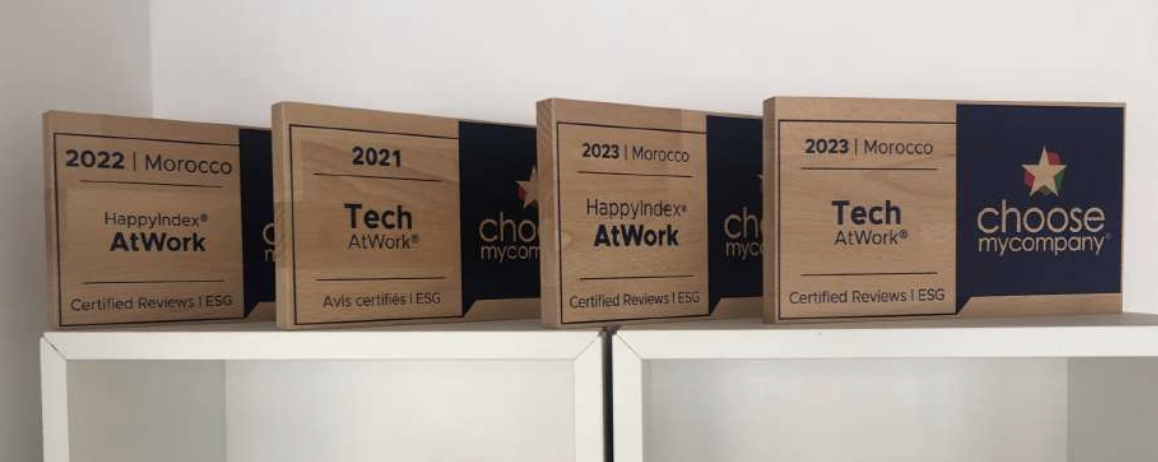
\includegraphics[width=0.7\linewidth]{images/theodo-awards.png}
\caption{Awards received by Theodo from ChooseMyCompany for excellence in workplace satisfaction and technology environment in 2021, 2022, and 2023.}
\end{figure}



\section{Hiring Process}

Securing an internship opportunity at \textit{Theodo} was an exhilarating journey that encompassed various stages of assessment and interaction. Each step of the process was meticulously designed to evaluate not just my technical prowess but also my personal attributes and aspirations. Let me walk you through the immersive experience of the \textit{Theodo} interview process.
It all began with the initial step, a multiple-choice questionnaire (MCQ). This phase tested my proficiency in full-stack development, object-oriented programming (OOP), data structures, as well as my familiarity with programming languages such as C and Java. The MCQ, held on Wednesday, 18th October 2024, provided a comprehensive overview of my technical knowledge and aptitude.

Following the MCQ, I progressed to the second stage: the HR exchange. Scheduled for Tuesday, 5th November 2024, this segment provided a platform for me to not only showcase my technical competencies but also to delve into personal anecdotes and experiences. Through a series of questions, I had the opportunity to introduce myself, share insights into my motivations for pursuing a career in software engineering, and narrate projects I had undertaken beyond academic endeavors. Moreover, I discussed instances where I encountered challenges and elucidated on the strategies employed to overcome them, thereby highlighting my problem-solving abilities. Additionally, the HR exchange allowed me to inquire about Theodo and gain deeper insights into the company culture and ethos.

The subsequent phase, a logic test conducted via Google Meet on Monday, 11th
November 2024, presented a captivating puzzle that tested my analytical and critical thinking skills. The scenario posed a thought-provoking challenge rooted in logic and reasoning, culminating in a stimulating exercise that showcased my ability to tackle complex problems methodically.

As I progressed further, I encountered the Test-Driven Development (TDD) interview, scheduled for Wednesday, 20th November 2024. This segment entailed the application of the Red-Green-Refactor approach to the Bowling Game Kata, emphasizing the importance of iterative development and test-driven methodologies. Through this exercise, I demonstrated not only my technical proficiency but also my adherence to best practices in software development.

The subsequent stage involved an interview with the Chief Technology Officer (CTO) via Google Meet on Wednesday, 2nd December 2024. This segment encompassed a wide array of topics ranging from fundamental data structures like LinkedLists and binary trees to advanced concepts such as immutability and design patterns. Through coding challenges and theoretical inquiries, I elucidated my understanding of core concepts while showcasing my problem-solving abilities and technical acumen.

The penultimate phase of the interview process involved a face-to-face interaction with the COO at \textit{Theodo} headquarters on Friday, 6th December 2024. This segment provided an opportunity for me to present myself holistically, discussing not just my academic and professional pursuits but also my extracurricular activities and personal aspirations. Additionally, the COO interview facilitated a candid dialogue wherein I gained insights into \textit{Theodo}' vision and ethos while articulating my own career aspirations and alignment with the company's values.

Finally, the journey culminated in a comprehensive tour of the workspace and a fruitful discussion with \textit{Theodo}' head of growth, wherein I had the opportunity to address any lingering queries and solidify my understanding of the company's culture and growth trajectory.

In retrospect, the \textit{Theodo} internship interview process was not just an evaluative exercise but a transformative journey that provided valuable insights, fostered personal growth, and affirmed my passion for software engineering. Through each phase, I embraced challenges, showcased my skills, and forged meaningful connections, culminating in a rewarding experience that laid the foundation for future endeavors. As I embark on this new chapter with \textit{Theodo}, I am filled with excitement and gratitude for the opportunity to contribute, learn, and grow within this dynamic and innovative organization.


\section{Onboarding Processes}

Starting my internship at \textit{Theodo} was an immersive and exhilarating experience, designed to integrate new team members seamlessly into the company’s dynamic environment. The onboarding process was comprehensive, fostering both professional growth and personal connections while ensuring that interns were well-equipped to contribute effectively from day one.

The journey began with the Asakai meeting, a hallmark of \textit{Theodo}' collaborative culture. On the very first day, I joined fellow interns in introducing ourselves to the team. The meeting was a vibrant mix of energy and enthusiasm, as each team showcased their progress. This initial introduction not only made us feel welcome but also provided insight into the ongoing projects and the company’s dynamic workflow. The morning concluded with a delightful breakfast in the office kitchen, offering a perfect opportunity to engage informally with team members and further build rapport.

\textit{Theodo} extended a warm welcome with some thoughtful swag, including branded merchandise that made us feel part of the team. We were also provided with official organization emails, granting access to professional accounts and the company's Notion page. This digital workspace was crucial for our onboarding, presenting tasks organized on a Kanban board, which we dived into for the rest of the day. These initial tasks were designed to familiarize us with the company’s tools and methodologies, setting a solid foundation for our roles.

The onboarding project provided a hands-on experience that was both challenging and rewarding. I delved into frontend development using Next.JS, exploring styled components alongside the MUI component library. Implementing the Redux pattern to dynamically toggle the theme mode and mastering various React hooks such as useState, useEffect, useRef, and useMemo were significant milestones. Additionally, creating custom hooks and leveraging existing ones from \textit{Theodo}’ boilerplate enhanced my understanding of efficient coding practices. An exciting aspect of this phase was testing UI components using the React Testing Library and Jest, culminating in the successful implementation of the landing and sign-in pages complete with all
necessary UI components.

Transitioning to backend development, my primary focus was on understanding and
utilizing the Spring Boot boilerplate. Initially, this posed a challenge, but as I became more familiar with its architecture, my productivity increased. The task of refactoring the existing codebase to align with the onboarding project’s requirements was meticulous but crucial, involving not just revamping code segments but also fine-tuning tests to ensure seamless functionality.

Throughout the onboarding process, I participated in several sessions and workshops that were pivotal for my professional development. Sessions with \textit{Kabous Nada} covered critical topics such as Andon, Perfect User Story, and Daily Mail, enhancing my understanding of effective project management and communication. Dojos and workshops provided deeper insights into various technical and methodological aspects, from standards of delivery to technical refinement and ticket manufacturing flow.

The onboarding process at \textit{Theodo} was a comprehensive and enriching experience. It was meticulously designed to integrate new interns into the company culture, equip them with essential tools and knowledge, and provide opportunities for meaningful contributions. This process not only prepared me for my role as a Software Engineer but also fostered a sense of belonging and collaboration, essential for my professional growth and success within the company.

Having established the organizational foundation and my integration into Theodo's collaborative environment, the following sections examine the specific project context and challenges that defined the FDME modernization initiative.

\newpage

\section{Project Context}

\subsection{Federation Structure and Scale}

The federation operates through a sophisticated hierarchical structure that reflects the diverse nature of national handball. At the national level, the federation oversees elite competitions including the Premier Men's Professional League, Elite Women's Professional League, and various national cup competitions. These high-profile events generate significant media attention and commercial value, requiring precise data management for broadcasting partners, sponsors, and regulatory compliance.

Regional committees manage intermediate-level competitions and coordinate with departmental committees who oversee local leagues and youth development programs. This three-tier structure ensures that handball remains accessible at the grassroots level while maintaining pathways for talented players to progress to elite levels. Each level has distinct reporting requirements, match formats, and regulatory frameworks that the FDME system must accommodate.

The federation also manages specialized competitions including beach handball, wheelchair handball, and corporate handball leagues, each with unique rules, scoring systems, and participant categories. This diversity demands a flexible, extensible platform capable of adapting to different sporting contexts while maintaining data consistency and integrity across all formats.

\subsection{Stakeholder Diversity and Workflow Complexity}

The FDME system serves an remarkably diverse user base, each with distinct needs, technical capabilities, and operational contexts:
Match Officials and Referees: Approximately 8,000 certified referees nationwide use the FDME during live matches. They require intuitive interfaces for real-time event recording, clear visual feedback for rule enforcement, and reliable offline operation since many gymnasiums lack stable internet connectivity. Referees often work under intense pressure during high-stakes matches, making usability and reliability paramount concerns.

\textbf{Club Administrators and Secretaries}: Volunteer administrators at the club level manage team registrations, player lineups, and pre-match preparations. Many are not technically sophisticated users and rely on clear, step-by-step workflows. They need efficient tools for roster management, player verification, and match result validation that don't require extensive training or technical support.

\textbf{Coaches and Team Staff}: Professional and amateur coaches use the system to verify player eligibility, track substitutions, and access real-time match statistics. They require mobile-friendly interfaces that work pitch-side and provide quick access to critical information during matches.

\textbf{Federation Officials}: Federation administrative staff require comprehensive tools for match oversight, data validation, dispute resolution, and regulatory compliance. They need detailed audit trails, bulk data processing capabilities, and integration with existing federation systems.

\textbf{Media and Broadcasting Partners}: Journalists, television broadcasters, and digital media platforms consume match data for live coverage, statistics compilation, and content creation. They require reliable, real-time data feeds and standardized formats for integration with their publishing systems.

\subsection{Digital Infrastructure Challenges}

The federation's digital infrastructure reflects decades of organic growth, with multiple systems developed at different times using varying technologies and standards. SportAdmin, the core federation management system, contains comprehensive member databases, competition structures, and historical records dating back many years. However, its architecture was designed for centralized, office-based administration rather than distributed, real-time match reporting.

This created a fundamental tension: match data needed to be captured in real-time across thousands of venues with varying connectivity, then integrated into a centralized system designed for batch processing and administrative workflows. The legacy FDME attempted to bridge this gap but struggled with the complexity of these requirements as the federation's operations expanded and user expectations evolved.

\section{Existing Legacy System Analysis}

\subsection{Historical Context and Evolution}

The original FDME was developed in the early 2010s when smartphone adoption was still emerging and most match reporting occurred on dedicated handheld devices or laptop computers. The system was built around Windows desktop applications with limited web interfaces, reflecting the computing landscape of its era. Over fifteen years of incremental development, the codebase had accumulated technical debt, compatibility issues, and user experience inconsistencies that made maintenance increasingly difficult and expensive.

The system's architecture reflected single-developer maintenance—a critical vulnerability that left the federation dependent on one person's knowledge and availability. Documentation was limited, testing procedures were manual, and deployment processes were ad-hoc, creating significant risks for an organization managing thousands of matches weekly

\begin{figure}[h]
\centering
\vspace{2em}
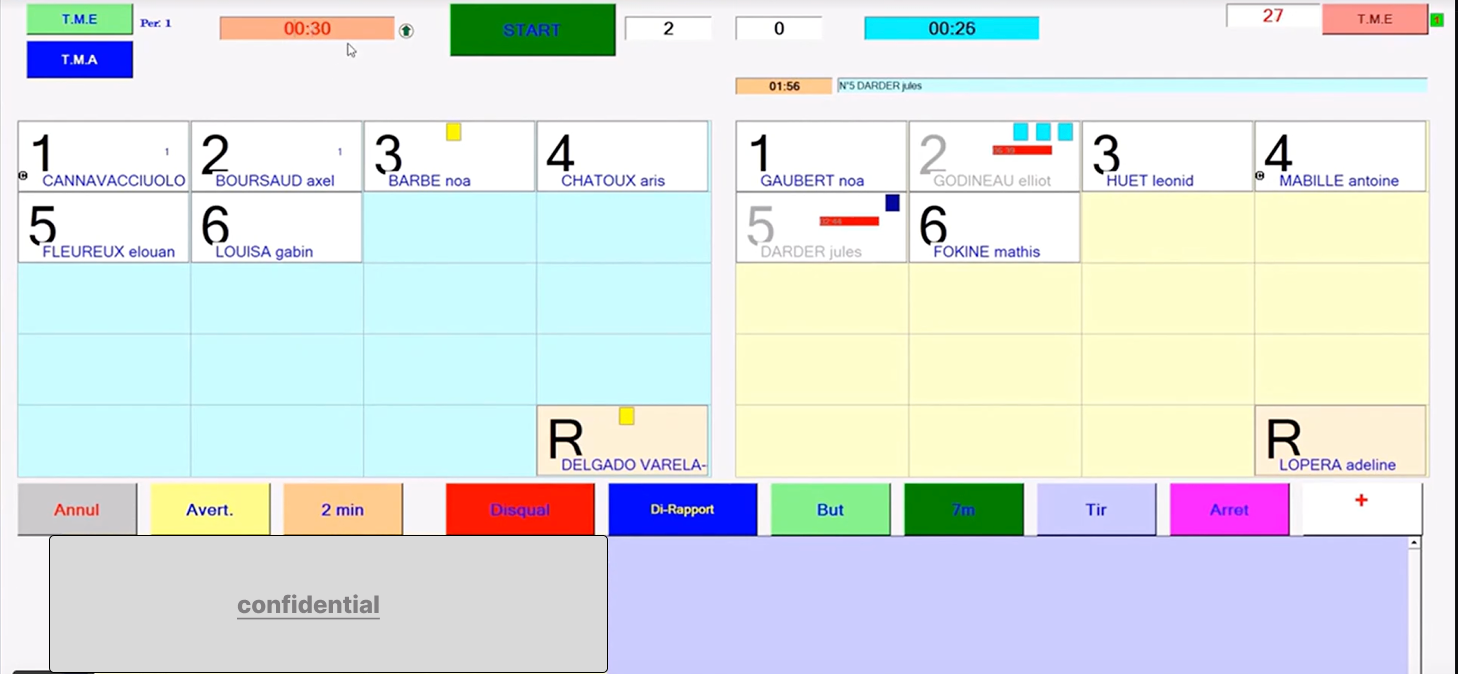
\includegraphics[width=12cm]{./images/legacy-system.png}
\caption{FDME Legacy App}
\end{figure}

\subsection{Technical Limitations and Performance Issues}

By 2025, the legacy FDME's technical limitations had become critical bottlenecks:
Platform Compatibility: The system required specific Windows versions and browser configurations that were increasingly difficult to maintain across the federation's diverse hardware ecosystem. Clubs struggled with compatibility issues on older machines, while newer devices often lacked necessary legacy components.

\textbf{Connectivity Resilience}: The original architecture assumed reliable internet connectivity, which was rarely available in sports venues. When connections failed, data could be lost or corrupted, requiring manual intervention and creating significant administrative overhead.

\textbf{User Interface Limitations}: The interface was designed for desktop use with mouse and keyboard input, making it difficult to use on tablets or touch devices that had become standard in many venues. Small buttons, complex navigation paths, and poor mobile responsiveness frustrated users and slowed match operations.

\textbf{Data Integrity Risks}: Limited validation rules and offline synchronization issues occasionally resulted in data inconsistencies, duplicate entries, or missing information that required manual correction by federation staff.

\textbf{Performance Degradation}: As match data volumes grew and user concurrency increased during peak weekend periods, the system experienced frequent slowdowns, timeouts, and crashes that disrupted live match operations.

\subsection{Real-World Operational Impact}

These technical limitations translated into tangible operational challenges that affected all stakeholders:

\textbf{Match Day Disruptions}: System failures during live matches created tense situations where referees couldn't record events, coaches couldn't verify player eligibility, and match results were delayed or lost entirely. In professional matches with television coverage, these delays could disrupt broadcast schedules and create contractual complications.

\textbf{Administrative Overhead}: Federation staff spent significant time manually resolving data inconsistencies, investigating missing match reports, and providing technical support to frustrated users. This reactive workload prevented investment in proactive improvements and strategic initiatives.

\textbf{User Frustration and Resistance}: Volunteers and officials increasingly expressed reluctance to use the system, with some reverting to paper-based processes that created additional manual data entry work for federation staff. This resistance threatened the federation's digital transformation goals and data quality objectives.

\textbf{Competitive Disadvantage}: While other national federations modernized their digital infrastructure, the federation's aging systems limited their ability to provide real-time statistics, enhanced broadcasting capabilities, and modern fan engagement features that had become standard in professional sports.


\subsection{Security and Compliance Concerns}

The legacy system's security architecture was designed for a different threat landscape and no longer met modern cybersecurity standards:

\textbf{Authentication Weaknesses}: Simple username/password authentication without multi-factor options created vulnerabilities, especially when credentials were shared among volunteers or stored insecurely.

\textbf{Audit Trail Limitations}: Insufficient logging and audit capabilities made it difficult to investigate data discrepancies, verify match results, or demonstrate compliance with regulatory requirements.



\section{Conclusion}

This chapter has established the comprehensive foundation necessary for understanding both the organizational excellence at Theodo Morocco and the complex challenges that necessitated the FDME modernization project. The intersection of Theodo's core values—rigor, pragmatism, eagerness to progress, and team spirit—with the federation's urgent need for digital transformation created an ideal environment for applying cutting-edge software engineering practices to challenges of national significance.
Theodo's evolution from Nimbleways into a key delivery hub within the international Theodo Group demonstrates the company's commitment to technical excellence and collaborative innovation. The comprehensive hiring process, from technical assessments through cultural alignment evaluation, and the structured onboarding experience reflect the organization's dedication to fostering professional growth while maintaining the highest standards of software delivery. These processes directly influenced how the FDME project was approached, ensuring that every team member was equipped with both the technical capabilities and collaborative mindset necessary for success.

The analysis of the National Sports Federation's operational scale—managing over 500,000 licensed members across 2,300 clubs and orchestrating more than 70,000 matches annually—reveals the critical importance of reliable digital infrastructure in modern sports administration. The federation's hierarchical structure, from elite professional leagues to grassroots youth development, creates complex reporting requirements that demand flexible, extensible technological solutions capable of adapting to diverse sporting contexts while maintaining data consistency and regulatory compliance.

The comprehensive examination of the legacy FDME system's limitations provides clear justification for the modernization initiative. From platform compatibility issues and connectivity resilience problems to user interface constraints and security vulnerabilities, the technical debt accumulated over fifteen years had created tangible operational challenges affecting every stakeholder in the handball ecosystem. The documented impact—including match day disruptions, administrative overhead, user frustration, and competitive disadvantage—demonstrates how technical limitations can directly undermine organizational effectiveness and user satisfaction.

Most importantly, this chapter establishes how Theodo's methodical approach to software delivery perfectly aligned with the federation's need for reliable, user-centered solutions. The company's emphasis on stakeholder collaboration, iterative development, and quality assurance provided the ideal framework for tackling the complex requirements of modernizing mission-critical systems while maintaining operational continuity. This foundation sets the stage for the detailed methodology, technical implementation, and successful outcomes that follow in subsequent chapters.

\newpage

	
\renewcommand{\chaptername}{Chapitre}
\mychapter{Methodology \& Development Approach}{Quate.}

//Text
	% \chapter{Conception}
Dans cette partie, nous verrons l’analyse des différences dans l’interface du projet. Ce projet avait pour objectif de développer une application intuitive visant à optimiser l'expérience utilisateur.


\section{ Architecture de la solution JobAI}

L’architecture de JobAI suit une approche modulaire, distribuée et orientée services, articulée autour d’un front-end web React, d’un backend intelligent (LLMs), d’un stockage centralisé dans Firebase, d’une extension Chrome autonome, et d’un agent IA externe pour la postulation automatique. Chaque composant remplit un rôle spécifique et communique avec les autres via des appels API ou des flux de données asynchrones.
Schéma d'interaction entre les composants


\begin{figure}[H]
    \centering
    % \setlength{\fboxrule}{0.5pt} % Épaisseur de la bordure
    % \setlength{\fboxsep}{0pt} % Espace entre image et bordure
    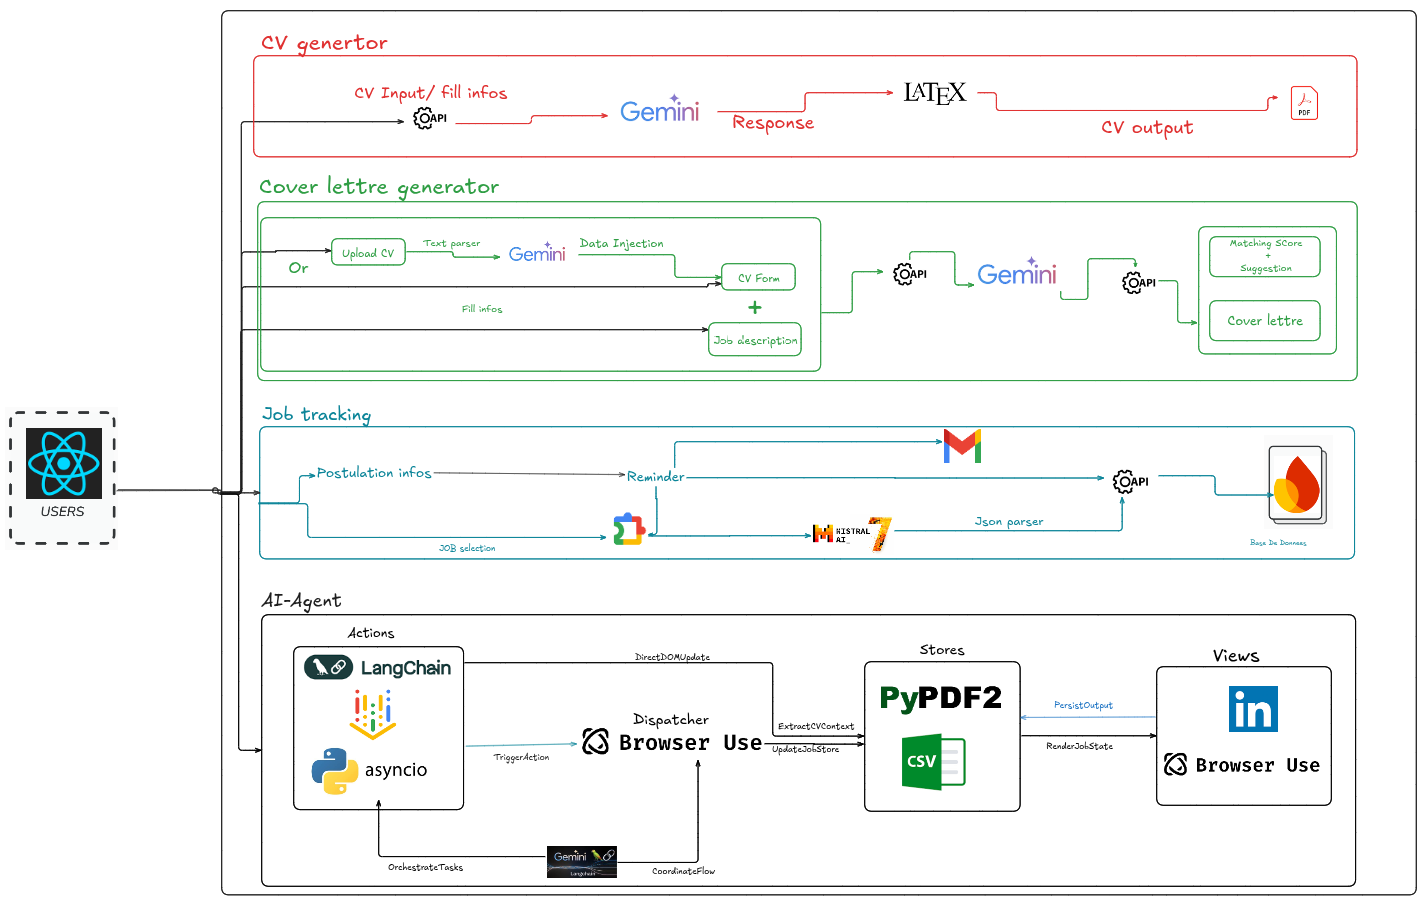
\includegraphics[width=1\linewidth]{screens/archi.png}
    \caption{Architecture de la solution}
    \label{fig: Architecture de la solution}
\end{figure}

\section*{Description détaillée des composants}

\begin{enumerate}
    \item \textbf{Interface Utilisateur Web – React.js + Tailwind CSS} \\
    Point d'entrée de l'utilisateur sur la plateforme JobAI permettant :\\
L'interface utilisateur web constitue le point d'entrée principal de l'utilisateur sur la plateforme JobAI. Développée avec React.js et stylisée avec Tailwind CSS, elle permet aux utilisateurs de renseigner manuellement leurs informations personnelles, expériences, compétences et préférences. Les utilisateurs peuvent également générer des CV ou lettres de motivation à partir des données saisies ou d'un CV importé. L'interface offre un tableau de bord intuitif pour consulter et suivre les candidatures, configurer les préférences de l'agent IA autonome, et interagir avec les modèles LLM à travers un design soigné et accessible.

    \item \textbf{Modèles de langage (LLMs)} \\
    Utilisés dans plusieurs processus clés :
Les modèles de langage sont utilisés dans plusieurs processus clés de la plateforme. Ils permettent la génération de CV à partir des informations fournies par l'utilisateur et la rédaction de lettres de motivation personnalisées selon l'offre d'emploi ciblée. Ces modèles réalisent également l'analyse sémantique permettant d'évaluer la compatibilité entre le profil du candidat et l'offre d'emploi, produisant un score de matching pertinent. Ils assurent aussi le parsing sémantique des descriptions d'offres capturées depuis l'extension, les structurant en format JSON exploitable. Ces modèles sont appelés via des fonctions backend ou microservices avec des prompts spécifiquement adaptés à chaque tâche.


    \item \textbf{Base de données cloud \& Authentification – Firebase} \\
    La base de données cloud Firebase constitue la brique centrale du stockage de l'application. Elle assure une authentification sécurisée via email/password ou OAuth et utilise Firestore pour stocker les données essentielles : profils utilisateurs, CV générés, lettres de motivation, offres sauvegardées et candidatures en cours. Cette infrastructure permet une gestion en temps réel des mises à jour concernant les offres, candidatures et logs de l'agent IA. Firebase offre une scalabilité naturelle et s'intègre de façon fluide avec React, simplifiant considérablement l'architecture technique de la solution.\\

    \item \textbf{Extension Chrome (JavaScript – Manifest V3)} \\
L'extension Chrome fonctionne comme un assistant embarqué directement dans le navigateur pour faciliter la collecte d'offres d'emploi. Elle propose une interface contextuelle qui s'active lors de la sélection d'offres sur des plateformes comme LinkedIn ou Indeed. L'extension extrait automatiquement les informations clés telles que le poste, l'entreprise et la localisation, puis envoie ces données à un backend LLM pour structuration en format JSON. Les offres sont ensuite sauvegardées dans Firebase sous l'espace personnel de l'utilisateur, permettant ainsi une centralisation rapide des opportunités professionnelles sans effort manuel significatif.\\


    \item \textbf{Agent IA autonome – Python + useBrowser} \\
L'agent IA autonome représente l'élément le plus innovant de la plateforme. Développé avec Python et la technologie useBrowser, il permet une navigation automatique sur des plateformes comme LinkedIn via un navigateur headless. Cet agent récupère les offres correspondant aux préférences définies par l'utilisateur, génère des candidatures complètes incluant CV et lettre de motivation adaptés, et peut même remplir automatiquement les formulaires pour postuler. Toutes les tentatives de postulation, qu'elles soient réussies ou non, sont journalisées dans Firebase pour assurer un suivi transparent. Son fonctionnement repose sur useBrowser qui combine efficacement l'automatisation du navigateur et les capacités des LLM.\\

    \item \textbf{Avantages de cette architecture}\\
Cette architecture présente de nombreux avantages stratégiques. Sa modularité permet une évolution ou un remplacement indépendant des composants, comme une éventuelle migration de Firebase vers MongoDB si nécessaire. La scalabilité est assurée par un backend cloud et des fonctions IA capables de monter en charge facilement selon les besoins. L'expérience utilisateur reste fluide grâce à la combinaison judicieuse d'automatisation, d'intelligence artificielle et de simplicité d'utilisation. Enfin, l'extensibilité de la plateforme permet d'envisager l'ajout d'autres agents pour des plateformes supplémentaires comme Indeed ou Welcome to the Jungle, élargissant ainsi progressivement sa couverture du marché de l'emploi.\\

\end{enumerate}

\section{Cas d'utilisation – Vue globale}
% \vspace{-1cm}
\begin{figure}[H]
    \centering
    \setlength{\fboxrule}{1pt} % Épaisseur de la bordure
    \setlength{\fboxsep}{0pt} % Espace entre image et bordure
    \fbox{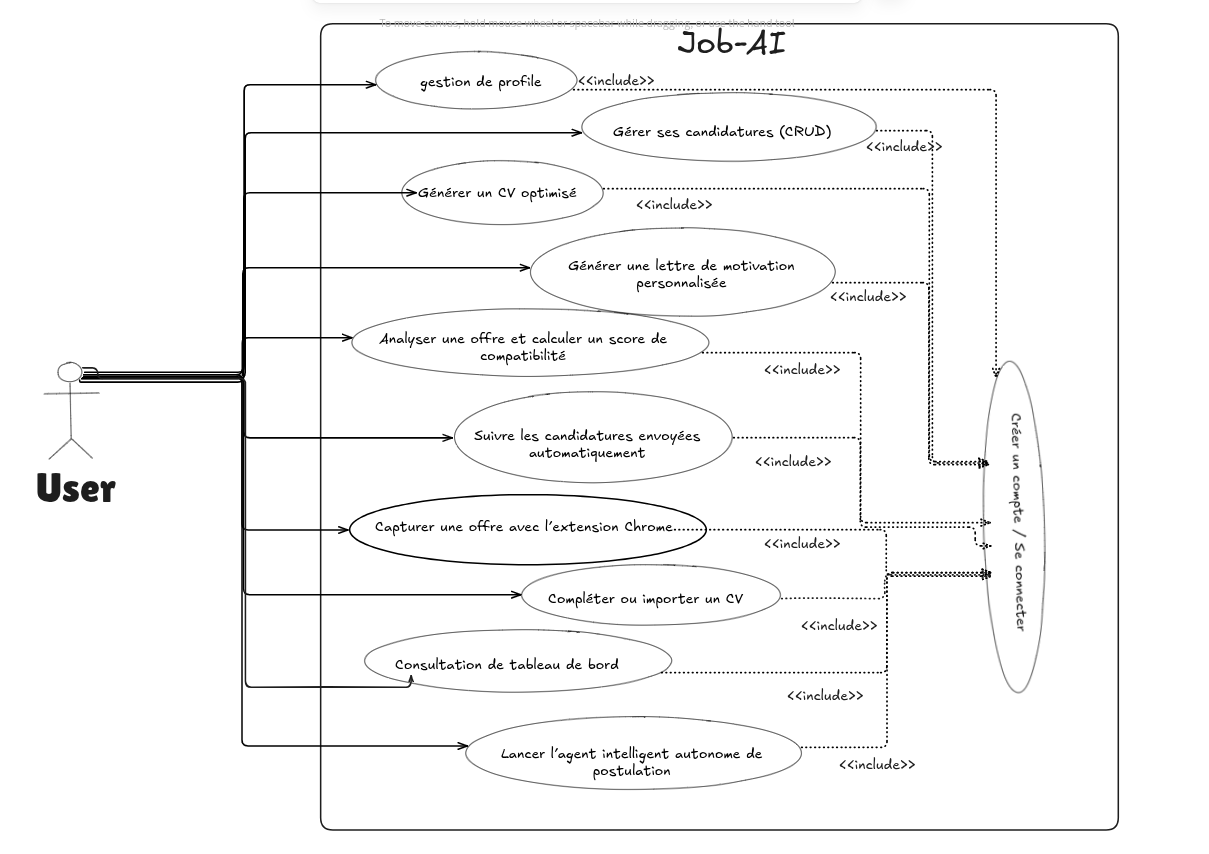
\includegraphics[width=0.8\linewidth]{screens/UseCase.png}}
    \caption{Diagramme des cas d'utilisation de JobAI}
    \label{fig:use_case}
\end{figure}


\begin{enumerate}
    \item \textbf{Créer un compte / Se connecter}
    \begin{itemize}
        \item \textbf{Objectif} : Accéder aux fonctionnalités personnalisées
        \item \textbf{Flux} :
        \begin{itemize}
            \item Inscription via email/mot de passe (Firebase Auth) ou SSO (Google/GitHub)
            \item Validation de l'email
        \end{itemize}
    \end{itemize}

    \item \textbf{Compléter ou importer un CV}
    \begin{itemize}
        \item \textbf{Flux} :
        \begin{itemize}
            \item Import : Téléversement d'un PDF $\rightarrow$ extraction automatique des données
            \item Édition manuelle : Ajout/suppression d'expériences, compétences, formations
        \end{itemize}
    \end{itemize}

    \item \textbf{Générer un CV optimisé}
    \begin{itemize}
        \item \textbf{Déclencheur} : Besoin d'adapter son CV à une offre spécifique
        \item \textbf{Flux} :
        \begin{itemize}
            \item Sélection d'un modèle
            \item Analyse des mots-clés de l'offre $\rightarrow$ suggestions d'optimisation (score ATS)
            \item Génération en PDF avec prévisualisation
        \end{itemize}
    \end{itemize}

    \item \textbf{Analyser une offre et calculer un score de compatibilité}
    \begin{itemize}
        \item \textbf{Flux} :
        \begin{itemize}
            \item Extraction des compétences/requis $\rightarrow$ comparaison avec le profil utilisateur
            \item Affichage d'un score \% (ex: "90\%")
            \item Suggestions pour améliorer la compatibilité
        \end{itemize}
    \end{itemize}

    \item \textbf{Gérer ses candidatures (CRUD)}
    \begin{itemize}
        \item \textbf{Objectif} : Suivre l'état des postulations
        \item \textbf{Flux} :
        \begin{itemize}
            \item Ajout : Manuel (formulaire) ou automatique (via extension/agent)
            \item Mise à jour : Changement de statut (ex: "Entretien prévu le 12/05")
            \item Rappel : Notifications email (Gmail API) selon dates configurées
            \item Suppression : Archivage ou suppression définitive
        \end{itemize}
    \end{itemize}

    \item \textbf{Capturer une offre avec l'extension Chrome}
    \begin{itemize}
        \item \textbf{Déclencheur} : Navigation sur un site d'emploi (Indeed, LinkedIn...)
        \item \textbf{Flux} :
        \begin{itemize}
            \item Clique sur l'extension $\rightarrow$ capture du titre, entreprise, description
            \item Pré-remplissage dans la plateforme $\rightarrow$ validation/édition par l'utilisateur
        \end{itemize}
    \end{itemize}

    \item \textbf{Lancer l'agent intelligent autonome de postulation}
    \begin{itemize}
        \item \textbf{Déclencheur} : Activation de l'automatisation pour une offre
        \item \textbf{Flux} :
        \begin{itemize}
            \item Paramétrage : CV/lettre par défaut, filtres (salaire, localisation)
        \end{itemize}
    \end{itemize}

    \item \textbf{Suivre les candidatures envoyées automatiquement}
    \begin{itemize}
        \item Auditer les candidatures automatiques et éviter les doublons
    \end{itemize}
\end{enumerate}

\textbf{Interconnexion des fonctionnalités} : \\
Les fonctionnalités sont accessibles depuis l'interface principale et interconnectées (ex: la génération de lettre nécessite un CV et/ou une offre).


\section{Diagramme de séquence – Génération de CV}

\begin{figure}[H]
    \centering
    \setlength{\fboxrule}{1pt} % Épaisseur de la bordure
    \setlength{\fboxsep}{0pt} % Espace entre image et bordure
    \fbox{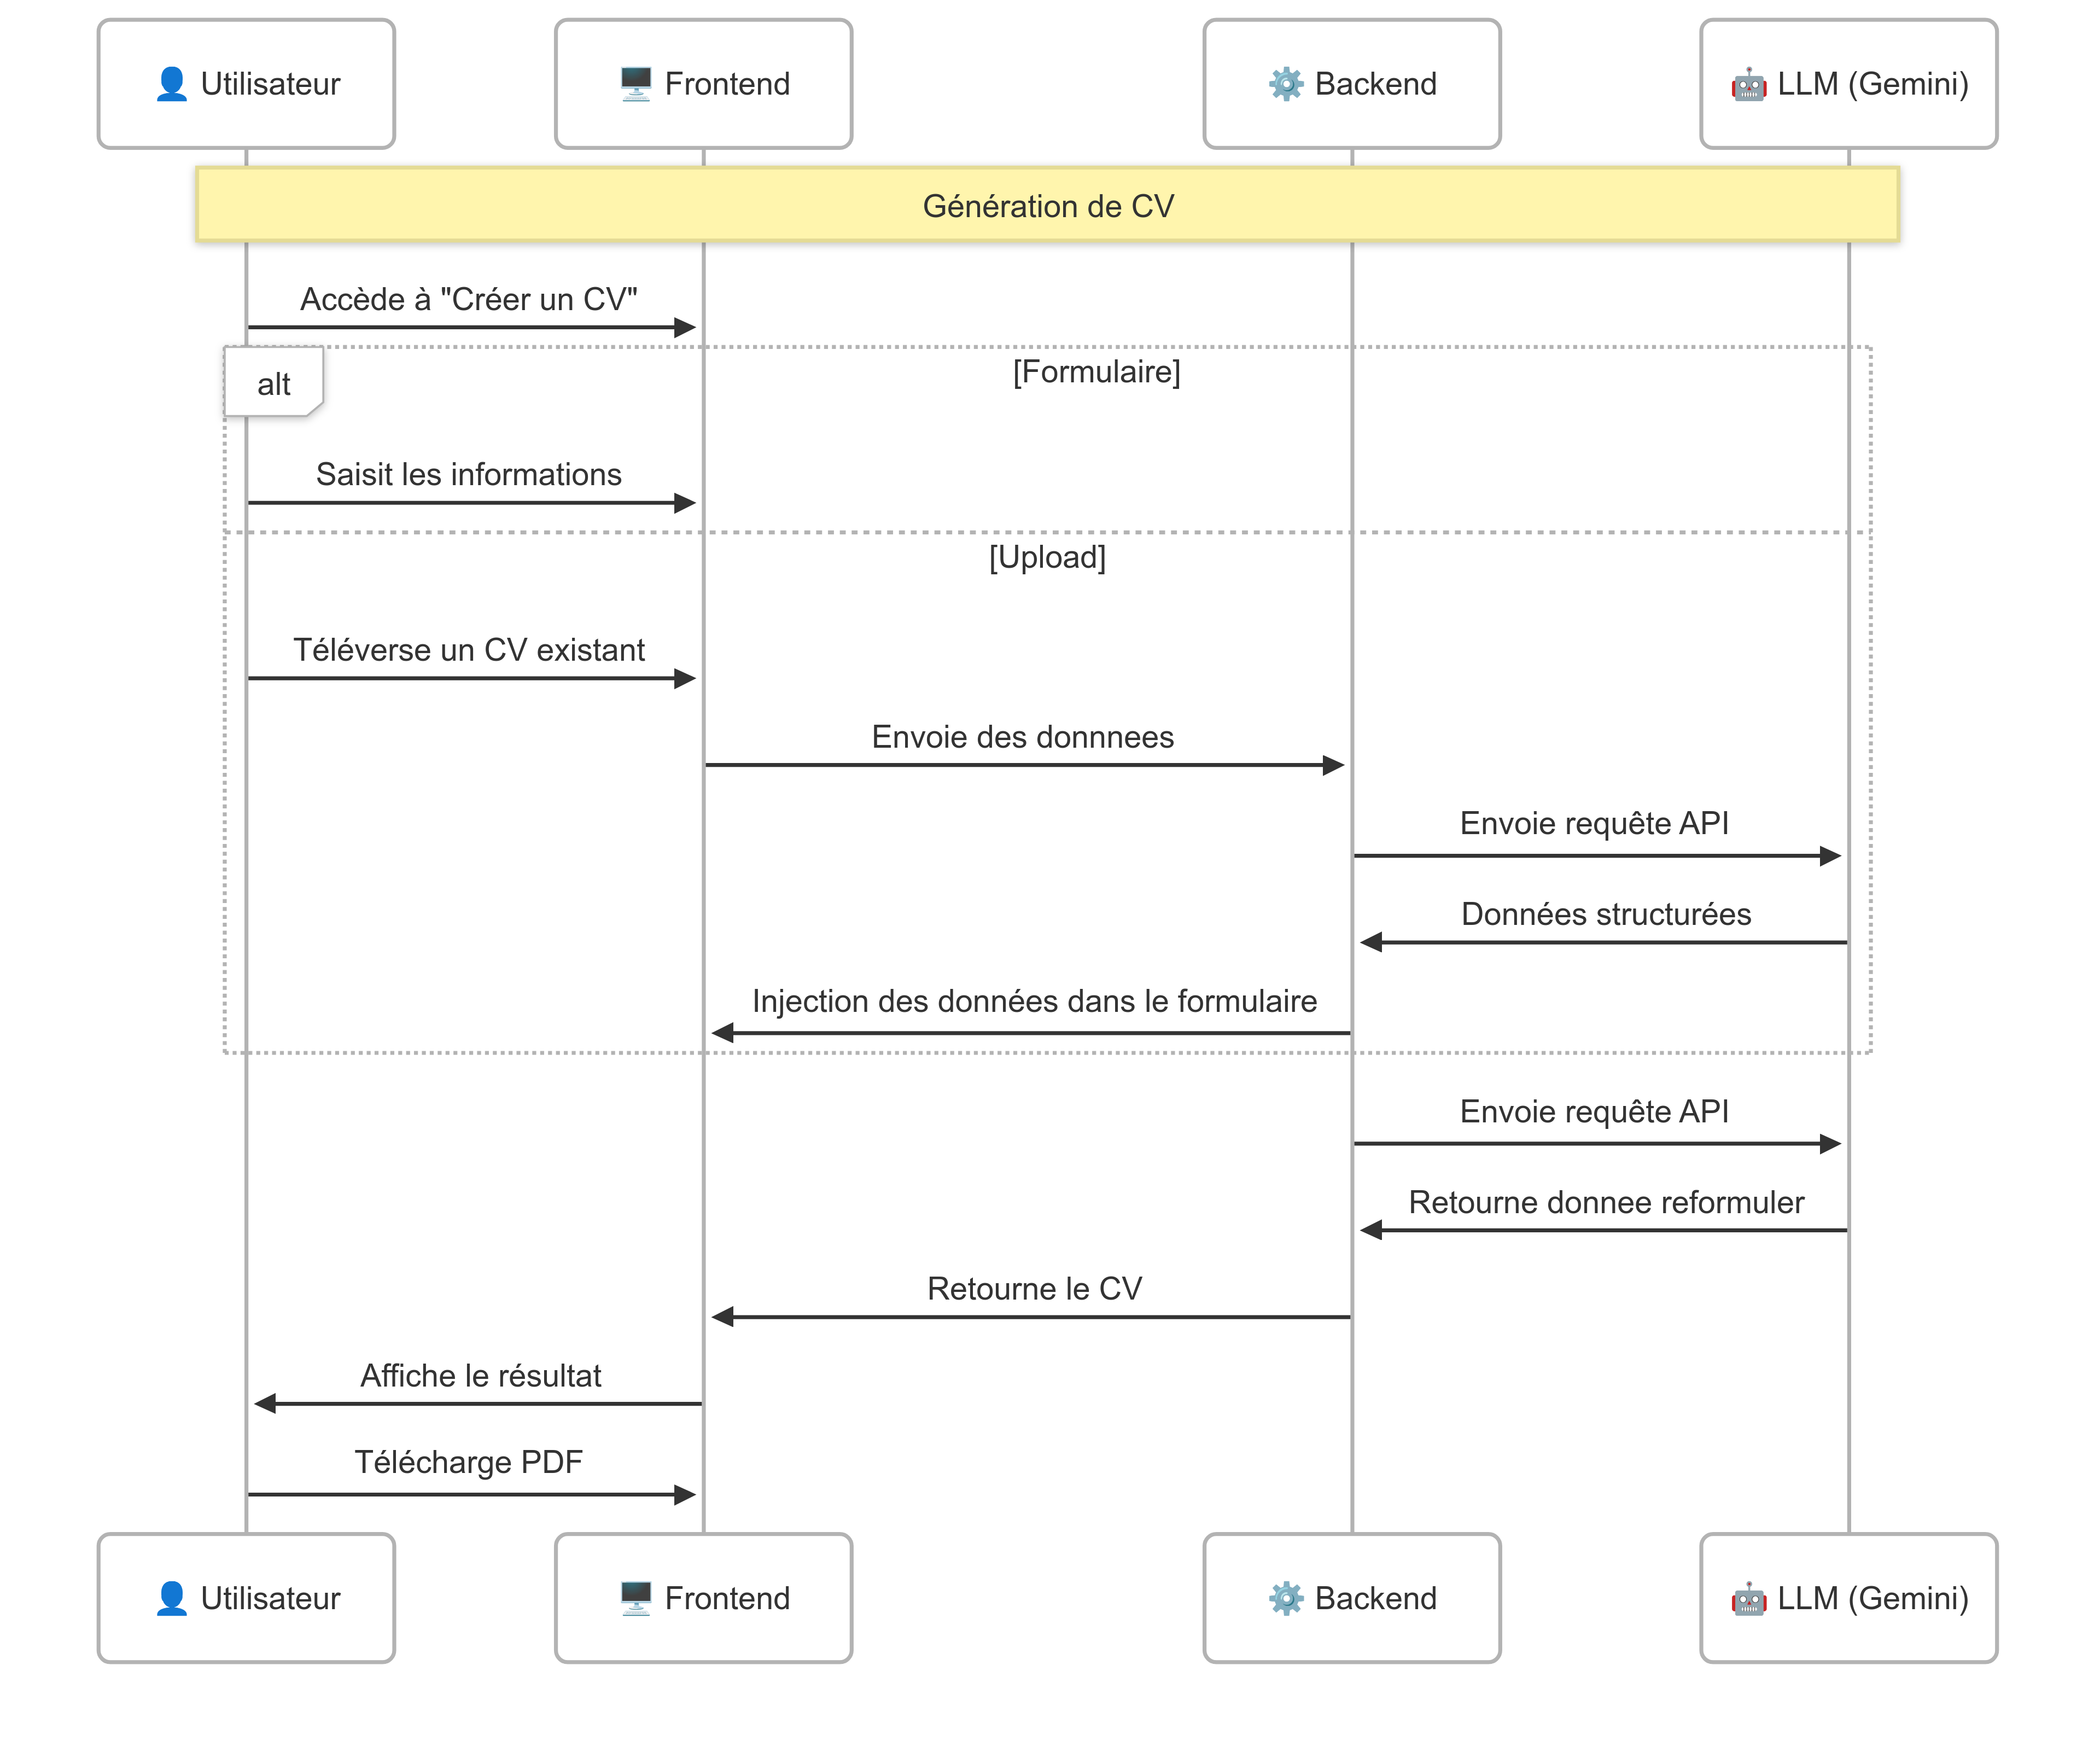
\includegraphics[width=1\linewidth]{screens/sequence-CV.png}}
    \caption{Architecture de la solution}
    \label{fig:Architecture_de_la_solution}
\end{figure}

\subsection*{Acteurs}
\begin{itemize}
    \item Utilisateur
    \item Interface Frontend
    \item Service Backend
    \item Modèle LLM (API IA)
\end{itemize}

\subsection*{Étapes du scénario}
\begin{enumerate}
    \item L'utilisateur accède à la fonctionnalité \og Créer un CV \fg{} depuis le tableau de bord
    
    \item Il choisit entre :
    \begin{itemize}
        \item Remplir un formulaire manuellement

                \item Téléverser un CV existant
    \end{itemize}
    \item Le Frontend transmet les données saisies ou le fichier au Backend
    
    \item Le Backend transforme les données en prompt structuré pour l'API IA
    
    \item Appel au modèle LLM via requête API (Gemini)
    
    \item Le modèle IA retourne un CV formaté selon les bonnes pratiques
    
    \item Le résultat est retourné au Frontend pour visualisation
    
    \item L'utilisateur peut :
    \begin{itemize}
        \item Télécharger le CV généré
        \item L'utiliser directement pour postuler
    \end{itemize}
\end{enumerate}

\subsection*{Flux alternatif}
\begin{itemize}
    \item \textbf{Échec de génération} : Si le modèle LLM ne retourne pas de résultat valide :
    \begin{enumerate}
        \item Le Backend envoie une notification d'erreur au Frontend
        \item L'interface propose à l'utilisateur de réessayer ou de modifier ses données
    \end{enumerate}
    
    \item \textbf{Optimisation supplémentaire} : L'utilisateur peut demander :
    \begin{itemize}
        \item Une version plus concise
        \item Une adaptation à un secteur spécifique
        \item Une traduction dans une autre langue
    \end{itemize}
\end{itemize}
\clearpage
\section{Diagramme de séquence – Cover Lettre}
Ce cas d'usage détaille le processus de génération automatisée d'une lettre de motivation personnalisée en exploitant les informations du CV utilisateur et les détails d'une offre d'emploi spécifique.
\begin{figure}[H]
    \centering
    \setlength{\fboxrule}{1pt} % Épaisseur de la bordure
    \setlength{\fboxsep}{0pt} % Espace entre image et bordure
    \fbox{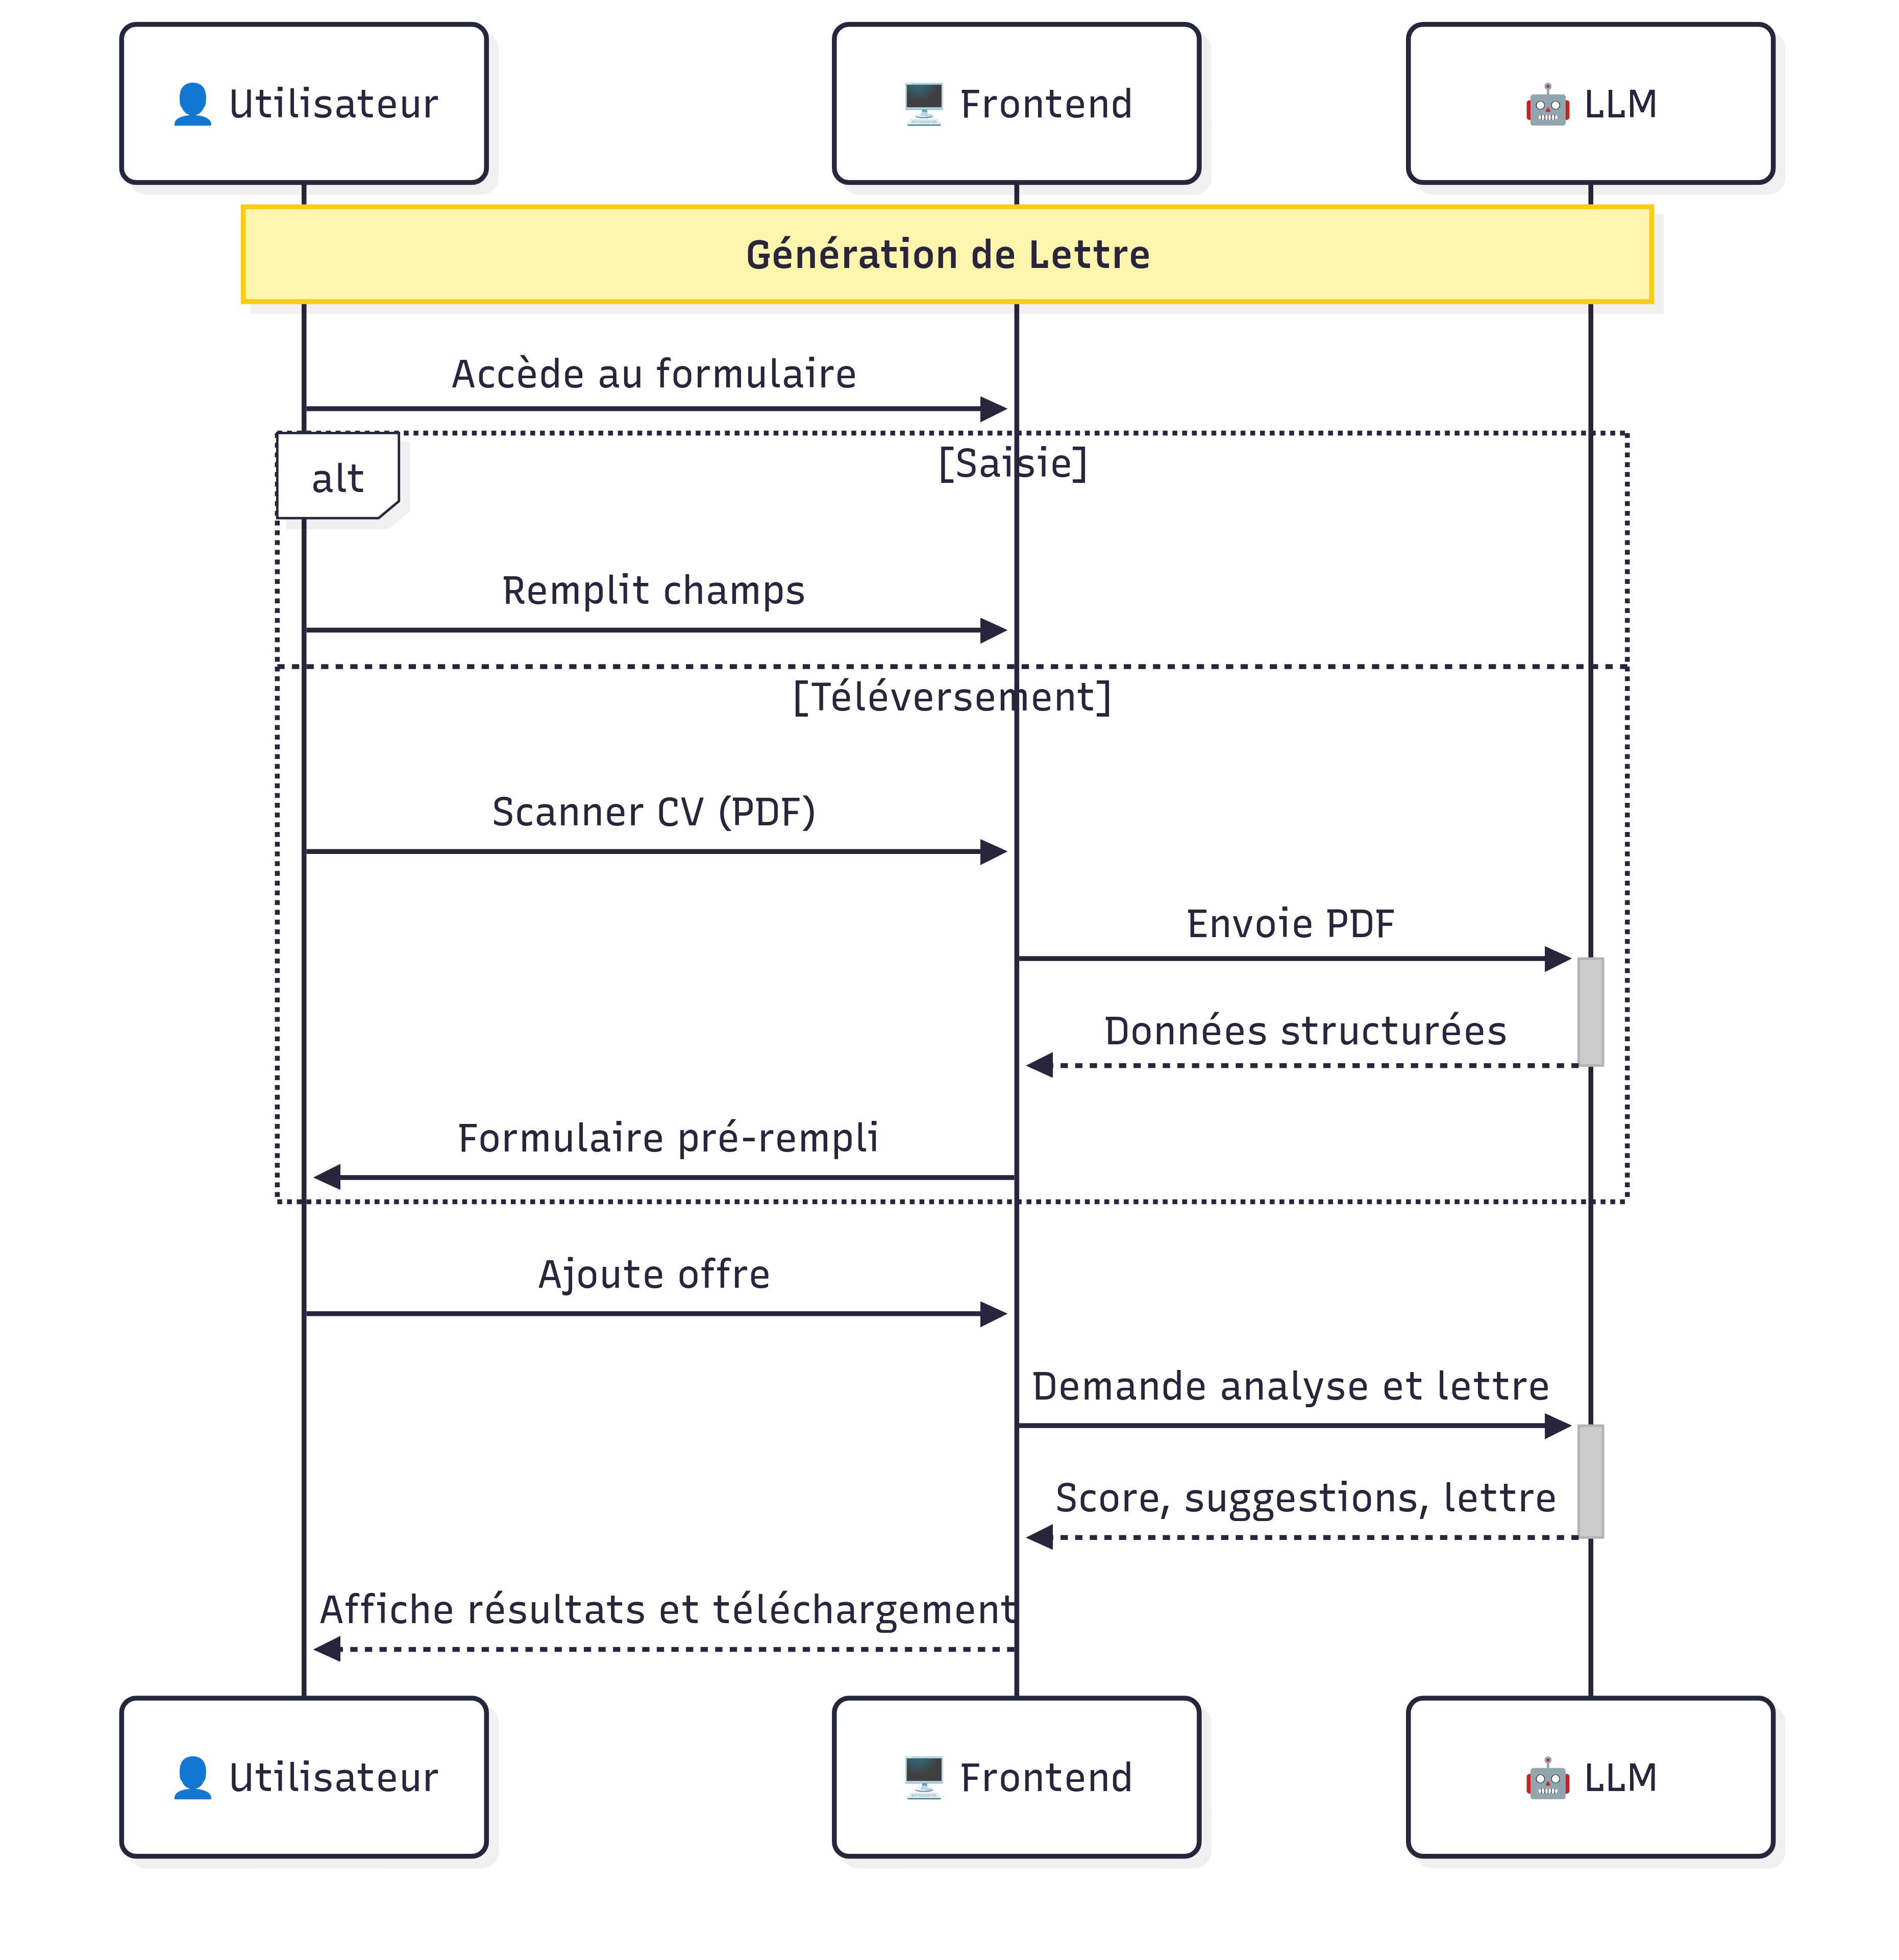
\includegraphics[width=0.8\linewidth]{screens/seqence-Lettre.png}}
    \caption{Architecture de la solution}
    \label{fig:Architecture_de_la_solution}
\end{figure}

\subsubsection*{Acteurs}
\begin{itemize}
    \item \textbf{Utilisateur} : Demandeur d'emploi souhaitant générer une lettre de motivation
    \item \textbf{Frontend} : Interface utilisateur web de la plateforme JobAI
    \item \textbf{Backend} : Service de traitement et orchestration des données
    \item \textbf{LLM} : Modèle de langage Gemini 1.5 Flash pour la génération de contenu
\end{itemize}

\subsubsection*{Prérequis}
\begin{itemize}
    \item L'utilisateur dispose d'un CV enregistré dans la plateforme
    \item Une offre d'emploi cible a été identifiée
    \item L'utilisateur est authentifié sur la plateforme
\end{itemize}

\subsubsection*{Étapes du scénario}

\begin{enumerate}
    \item L'utilisateur accède au module \og Génération de Lettre \fg{} depuis le tableau de bord principal
    
    \item Le système affiche le formulaire de génération avec les options suivantes :
    \begin{itemize}
        \item Saisie manuelle des informations de l'offre
        \item Téléversement d'un CV existant (PDF)
    \end{itemize}
    
    \item L'utilisateur choisit sa méthode préférée et renseigne les champs requis :
    \begin{itemize}
        \item \textbf{Si saisie manuelle} : remplissage du formulaire avec les détails de l'offre
        \item \textbf{Si téléversement} : sélection et upload du fichier CV (PDF)
    \end{itemize}
    
    \item Le Frontend transmet les données saisies au service Backend via une requête API sécurisée
    
    \item \textbf{Si CV téléversé} : Le Backend déclenche le processus de scan et d'extraction :
    \begin{itemize}
        \item Analyse du document PDF
        \item Extraction des données structurées (compétences, expériences, formation)
        \item Structuration des informations au format JSON
    \end{itemize}
    
    \item Le Backend prépare le formulaire pré-rempli en fusionnant :
    \begin{itemize}
        \item Les données extraites du CV
        \item Les informations de l'offre d'emploi
        \item Le profil utilisateur existant
    \end{itemize}
    
    \item L'utilisateur valide et complète les informations affichées dans le formulaire pré-rempli
    
    \item L'utilisateur ajoute les détails spécifiques de l'offre d'emploi cible (entreprise, poste, exigences)
    
    \item Le Frontend envoie l'ensemble des données validées au Backend pour traitement
    
    \item Le Backend formule une requête structurée vers l'API du modèle LLM incluant :
    \begin{itemize}
        \item Le prompt de génération de lettre de motivation
        \item Les données du profil candidat
        \item Les informations de l'offre d'emploi
        \item Les paramètres de personnalisation
    \end{itemize}
    
    \item Le modèle LLM analyse les données et génère :
    \begin{itemize}
        \item Une lettre de motivation personnalisée
        \item Un score de compatibilité profil/offre
        \item Des suggestions d'amélioration du profil
    \end{itemize}
    
    \item Le Backend reçoit la réponse du LLM et effectue les traitements suivants :
    \begin{itemize}
        \item Validation et formatage de la lettre générée
        \item Sauvegarde dans la base de données utilisateur
        \item Préparation des métadonnées (score, suggestions)
    \end{itemize}
    
    \item Le système affiche à l'utilisateur :
    \begin{itemize}
        \item La lettre de motivation générée avec prévisualisation
        \item Le score de compatibilité calculé
        \item Les suggestions d'optimisation personnalisées
        \item Les options de téléchargement (PDF, Word)
    \end{itemize}
    
    \item L'utilisateur peut :
    \begin{itemize}
        \item Télécharger la lettre au format souhaité
        \item Modifier le contenu avant téléchargement
        \item Sauvegarder pour usage ultérieur
        \item Générer une nouvelle version avec des paramètres différents
    \end{itemize}
\end{enumerate}

\subsubsection*{Résultats attendus}
\begin{itemize}
    \item Génération d'une lettre de motivation personnalisée et professionnelle
    \item Évaluation de la compatibilité entre le profil candidat et l'offre
    \item Recommandations pour améliorer l'adéquation du profil
    \item Document prêt à l'emploi disponible en plusieurs formats
\end{itemize}

\subsubsection*{Cas d'exception}
\begin{itemize}
    \item \textbf{Échec de scan PDF} : Message d'erreur et suggestion de saisie manuelle
    \item \textbf{Indisponibilité du LLM} : Notification à l'utilisateur et mise en file d'attente
    \item \textbf{Données insuffisantes} : Demande de complétion du profil utilisateur
\end{itemize}

% \begin{figure}
% 	\centering
% 	\begin{subfigure}[b]{0.45\textwidth}
% 		% \includegraphics[width=\textwidth]{screens/login.png}
% 		\caption{Page de connexion}
% 		\label{fig:login}
% 	\end{subfigure}
% 	\hfill
% 	\begin{subfigure}[b]{0.40\textwidth}
% 		% \fbox{\includegraphics[width=\textwidth]{screens/signup.png}}
% 		\caption{Page d'inscription}
% 		\label{fig:signup}
% 	\end{subfigure}
% 	\caption{Authentification utilisateur}
% 	\label{fig:auth}
% \end{figure}


	% \chapter{Realisation}
\section{Outils et technologies utilisés}

\noindent
\begin{minipage}{0.1\textwidth}
    
\includegraphics[height=3em]{LOGOS/React-icon.svg.png}
\end{minipage}%
\begin{minipage}{0.9\textwidth}
    \textbf{React.js} \\
    Bibliothèque JavaScript développée par Meta pour construire des interfaces utilisateur dynamiques à base de composants. \\
    \end{minipage}

\vspace{0.8em}
\noindent
\begin{minipage}{0.1\textwidth}
    
\includegraphics[height=3em]{LOGOS/Tailwind CSS.png}
\end{minipage}%
\begin{minipage}{0.9\textwidth}
    \textbf{Tailwind CSS} \\
    Framework CSS utility-first qui permet de construire rapidement des designs personnalisés. \\
   
\end{minipage}

\vspace{0.8em}
\noindent
\begin{minipage}{0.1\textwidth}
    
\includegraphics[height=3em]{LOGOS/Python.png}
\end{minipage}%
\begin{minipage}{0.9\textwidth}
    \textbf{Python} \\
    Langage de programmation principal pour le backend. \\
    \textit{Cas d'usage dans JobAI} : Développement du serveur Flask, traitement des données, intégration avec les APIs d'IA.
\end{minipage}


\vspace{0.8em}
\noindent
\begin{minipage}{0.1\textwidth}
    
\includegraphics[height=3em]{LOGOS/Flask.png}
\end{minipage}%
\begin{minipage}{0.9\textwidth}
    \textbf{Flask} \\
    Framework web léger pour Python. Création des API REST, gestion des routes, intégration avec les services d'IA.
\end{minipage}


\vspace{0.8em}
\noindent
\begin{minipage}{0.1\textwidth}
    
\includegraphics[height=3em]{LOGOS/Firebase.png}
\end{minipage}%
\begin{minipage}{0.9\textwidth}
    \textbf{Firebase} \\
     Nous avons utilisé Firebase pour stocker les utilisateurs, les documents générés, les candidatures et les préférences. Il gère aussi l’authentification sécurisée (login, signup) et héberge l’application web.
\end{minipage}


\vspace{0.8em}
\noindent
\begin{minipage}{0.1\textwidth}
    
\includegraphics[height=3em]{LOGOS/Chrome.png}
\end{minipage}%
\begin{minipage}{0.9\textwidth}
    \textbf{Extension Chrome (Manifest V3)} \\
    Une extension Chrome est un petit programme qui s’intègre au navigateur et permet d’interagir avec les pages web visitées. Le format Manifest V3 est la dernière norme de sécurité pour les extensions.
\end{minipage}

\vspace{0.8em}
\noindent
\begin{minipage}{0.1\textwidth}
    \includegraphics[height=3em]{LOGOS/GitHub.png}
\end{minipage}%
\begin{minipage}{0.9\textwidth}
    \textbf{GitHub} \\
    Plateforme de gestion de code source basée sur Git. Hébergement du code source, collaboration d'équipe et gestion des versions.
\end{minipage}

\vspace{0.8em}
\noindent
\begin{minipage}{0.1\textwidth}
    
\includegraphics[height=2.4em]{LOGOS/Trello.png} \\
    
\includegraphics[height=2.4em]{LOGOS/Notion.png}
\end{minipage}%
\begin{minipage}{0.9\textwidth}
    \textbf{Trello et Notion} \\
     Nous avons utilisé Trello ou Notion pour organiser les sprints hebdomadaires, suivre les tâches, noter les idées de fonctionnalités, et documenter les décisions techniques prises en cours de développement.
\end{minipage}


\vspace{0.8em}
\noindent
\begin{minipage}{0.1\textwidth}
    
\includegraphics[height=3em]{LOGOS/Gemini.png}
\end{minipage}%
\begin{minipage}{0.9\textwidth}
    \textbf{Gemini API} \\
   Nous avons utilisé l’API pour générer automatiquement des CV et lettres de motivation à partir de données utilisateur ou de fichiers importés, mais aussi pour analyser les offres et calculer un score de similarité avec le profil.\\
\end{minipage}

\subsection{Sélection du Modèle de Langage : Gemini Flash 1.5}


Le choix du modèle de langage constitue une décision stratégique cruciale pour JobAI, impactant directement la qualité des CV générés, l'expérience utilisateur et la viabilité économique du projet. Notre processus de sélection s'est appuyé sur une analyse comparative rigoureuse des principaux modèles disponibles sur le marché, en tenant compte de critères techniques, économiques et fonctionnels spécifiques à notre cas d'usage.

\begin{figure}[H]
    \centering
    \setlength{\fboxrule}{0.2pt} % Épaisseur de la bordure
    \setlength{\fboxsep}{0pt} % Espace entre image et bordure
    \fbox{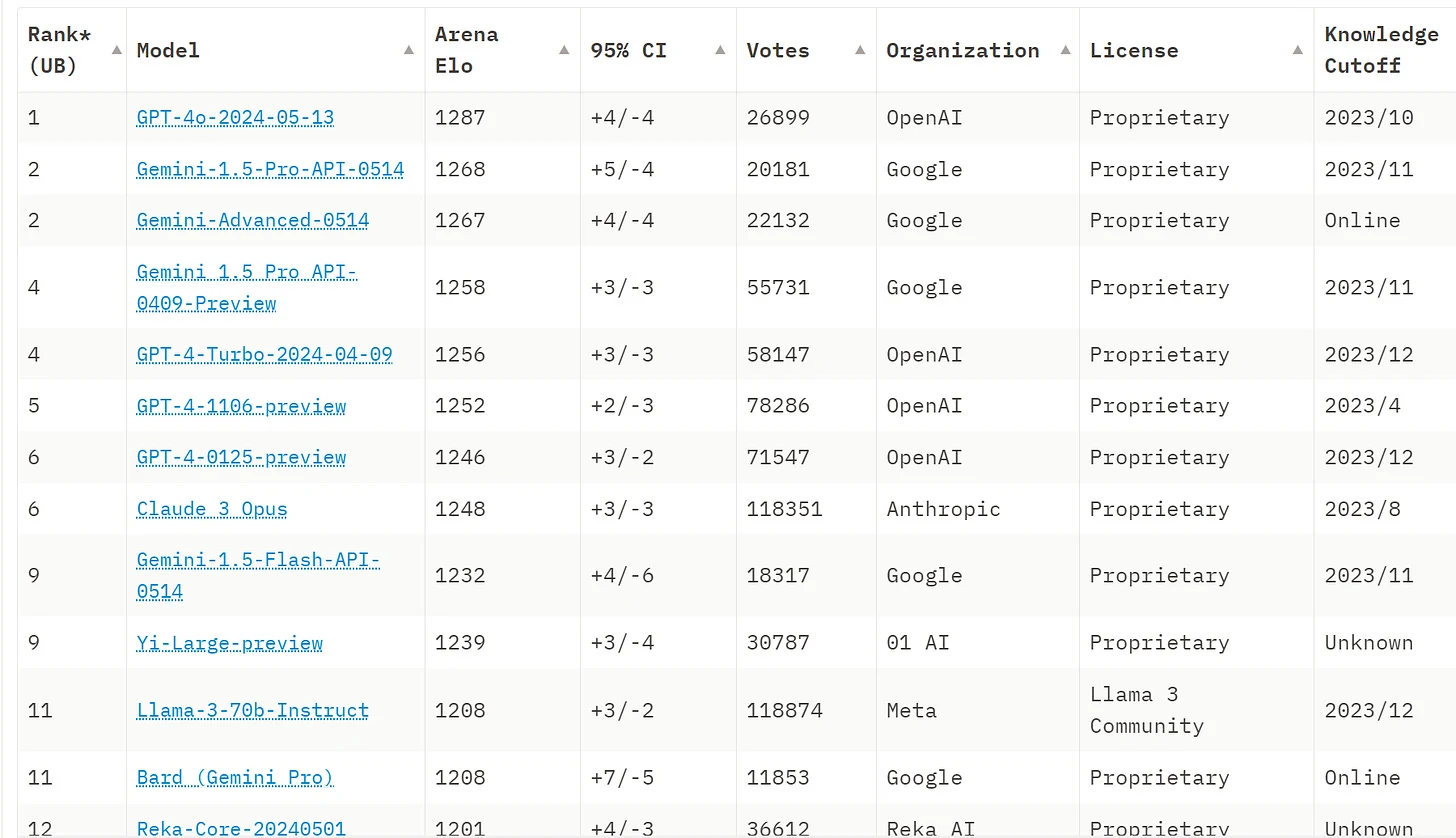
\includegraphics[width=1\linewidth]{screens/Benchmark.png}}
    \caption{Comparatif des performances des principaux modèles (Arena Elo Rankings)}
    \label{fig:llm_benchmark}
\end{figure}

\subsubsection{Critères de Sélection}

Notre évaluation s'est articulée autour de six critères fondamentaux :

\begin{enumerate}
    \item \textbf{Performance et Qualité} : Capacité à générer du contenu professionnel structuré et cohérent
    \item \textbf{Coût d'Utilisation} : Viabilité économique pour une application destinée au grand public
    \item \textbf{Vitesse de Traitement} : Latence acceptable pour une expérience utilisateur fluide
    \item \textbf{Capacité de Contexte} : Aptitude à traiter des informations professionnelles complexes
    \item \textbf{Accessibilité} : Disponibilité des API et facilité d'intégration
    \item \textbf{Écosystème} : Compatibilité avec les outils et services existants
\end{enumerate}

\subsubsection{Analyse Comparative des Modèles}

L'analyse du benchmark présenté en Figure \ref{fig:llm_benchmark} révèle plusieurs insights significatifs :

\paragraph{Modèles Premium} Les modèles GPT-4o et Gemini 1.5 Pro occupent les premières positions avec des scores Arena Elo supérieurs à 1250, démontrant des performances exceptionnelles. Cependant, leurs coûts d'utilisation élevés constituent un frein majeur pour notre application.

\paragraph{Modèles Intermédiaires} Claude 3 Opus et les variantes GPT-4 offrent un compromis intéressant entre performance et coût, mais restent dans une gamme tarifaire élevée pour un usage intensif.

\paragraph{Modèles Optimisés} Gemini 1.5 Flash se distingue par un positionnement unique, offrant des performances solides (score Arena Elo de 1232) tout en bénéficiant d'une politique tarifaire particulièrement attractive.

\subsubsection{Justification du Choix : Gemini 1.5 Flash}

Après évaluation approfondie, Gemini 1.5 Flash s'impose comme le choix optimal pour JobAI, réunissant les avantages suivants :

\begin{itemize}
    \item Score Arena Elo de 1232, attestant de capacités avancées en génération de contenu
    \item Fenêtre de contexte de 1 million de tokens, permettant le traitement d'informations professionnelles étendues
    \item Débit de 150+ tokens/seconde, assurant une réactivité optimale
    \item API gratuite dans les limites d'usage standard, éliminant les coûts d'exploitation initiaux
    \item Modèle économique adapté aux startups et projets étudiants
    \item API bien documentée et stable
    \item Support natif des formats de sortie structurés (JSON, XML)
\end{itemize}


Cette sélection représente un équilibre optimal entre performance technique, viabilité économique et facilité d'implémentation, constituant un fondement solide pour le développement de JobAI.

\subsubsection{Perspectives d'Évolution}

L'architecture modulaire de JobAI permet une évolution future vers des modèles plus performants si les contraintes budgétaires le permettent. Un système de basculement vers GPT-4o ou Gemini 1.5 Pro pourra être envisagé pour les utilisateurs premium, offrant ainsi une stratégie de monétisation progressive.
\newpage
\section{Les Interfaces de l'Application}

Cette section présente les principales interfaces de JobAI, conçues pour offrir une expérience utilisateur intuitive et complète dans la gestion de la recherche d'emploi. Chaque interface répond à des besoins spécifiques tout en maintenant une cohérence visuelle et fonctionnelle.

\subsection{Interface de Tableau de Bord}

\begin{figure}[H]
    \centering
    \setlength{\fboxrule}{0.2pt} % Épaisseur de la bordure
    \setlength{\fboxsep}{0pt} % Espace entre image et bordure
    \fbox{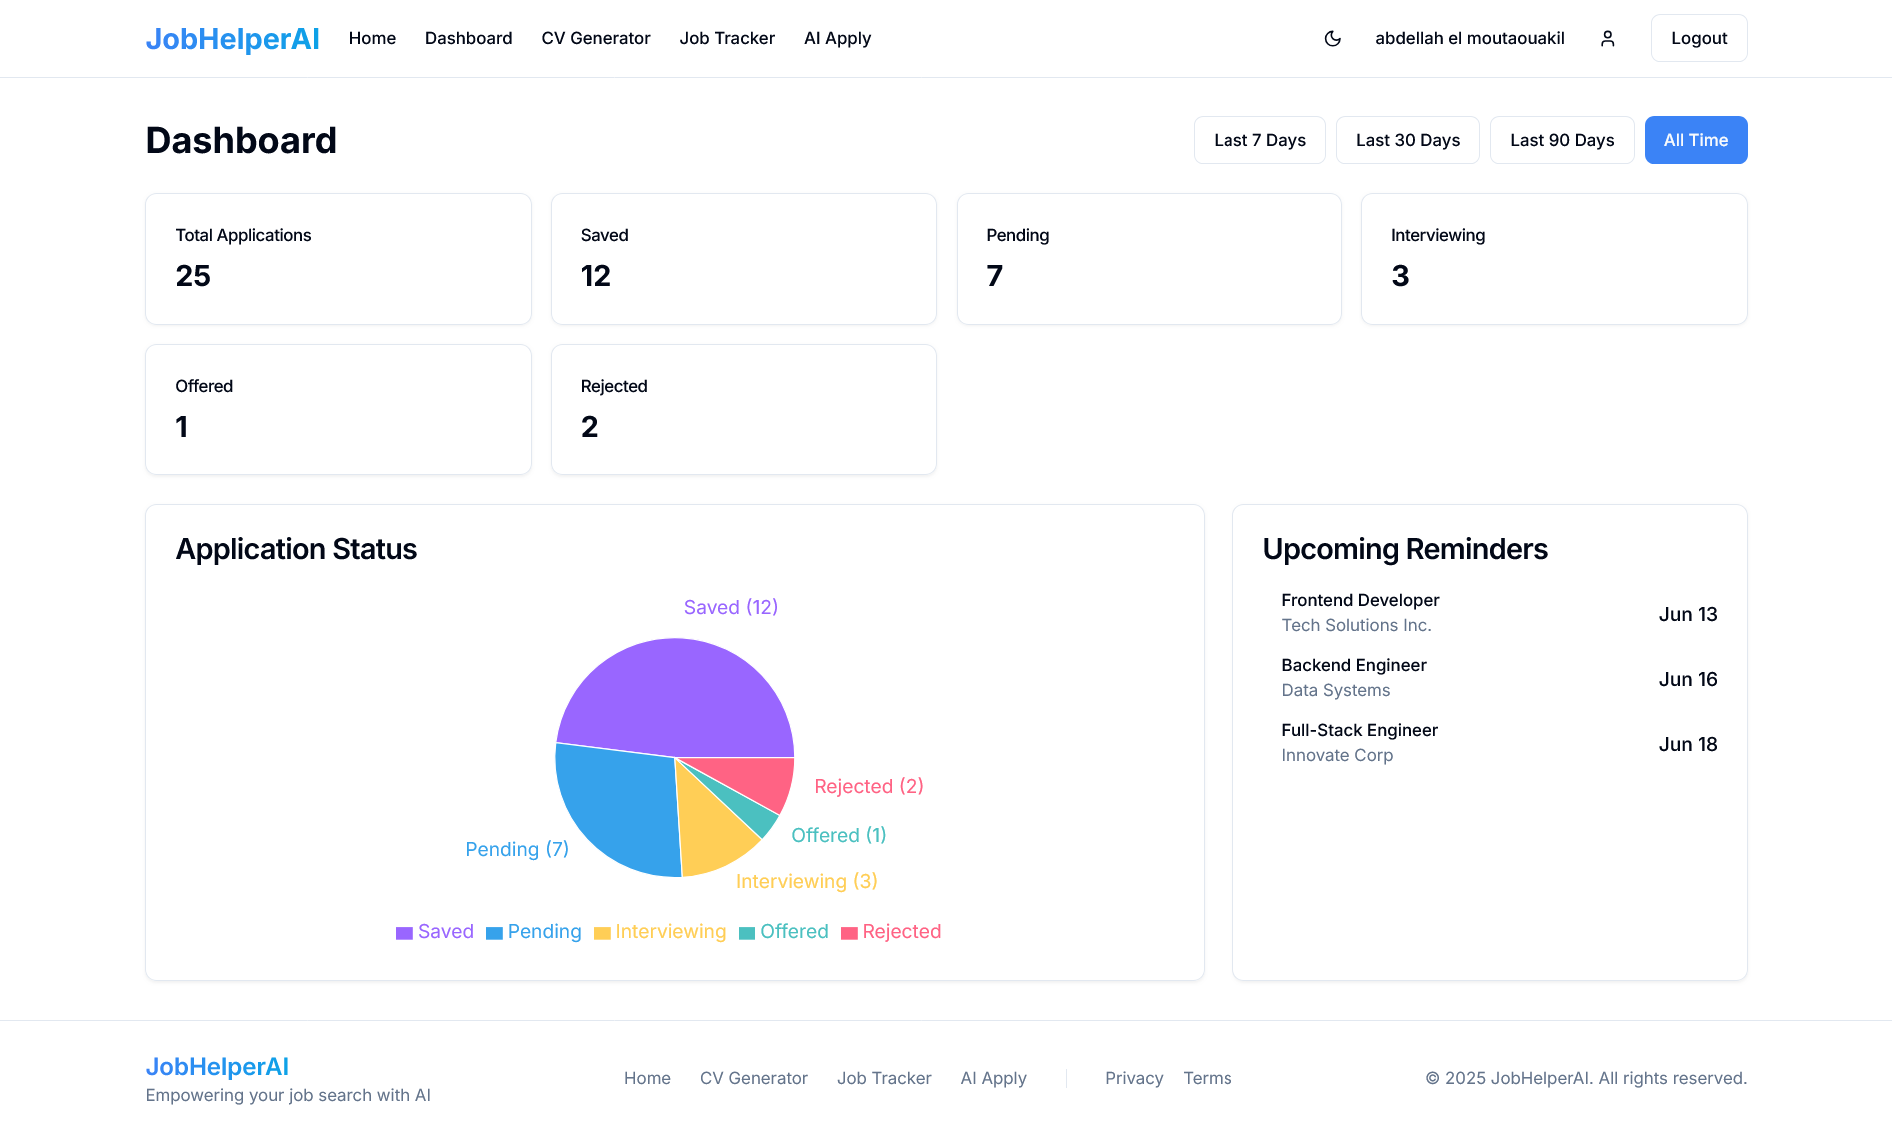
\includegraphics[width=1\linewidth]{screens/dashboard.png}}
    \caption{Interface du tableau de bord principal}
    \label{fig:dashboard}
\end{figure}

La page "Tableau de Bord" constitue le point central de l'application, offrant à l'utilisateur une vue d'ensemble synthétique et visuelle de ses activités de recherche d'emploi. Cette interface présente des statistiques clés concernant les candidatures, notamment le nombre total d'offres enregistrées et leur répartition par statut (en attente, entretien, refusé, accepté).\\

Un graphique interactif lui permet de visualiser rapidement l'état d'avancement de ses démarches, tandis qu'une section dédiée lui rappelle les prochaines échéances importantes. Grâce aux filtres temporels, l'utilisateur peut également analyser sa performance sur les 7, 30 ou 90 derniers jours, lui offrant ainsi un outil puissant pour suivre sa progression et ajuster sa stratégie.\\
\subsection{Gestion des Offres d'Emploi}

\subsubsection{Consultation des Offres}
\vspace{-0.5cm}
\begin{figure}[H]
    \centering
        \setlength{\fboxrule}{0.2pt} % Épaisseur de la bordure
    \setlength{\fboxsep}{0pt} % Espace entre image et bordure
    \fbox{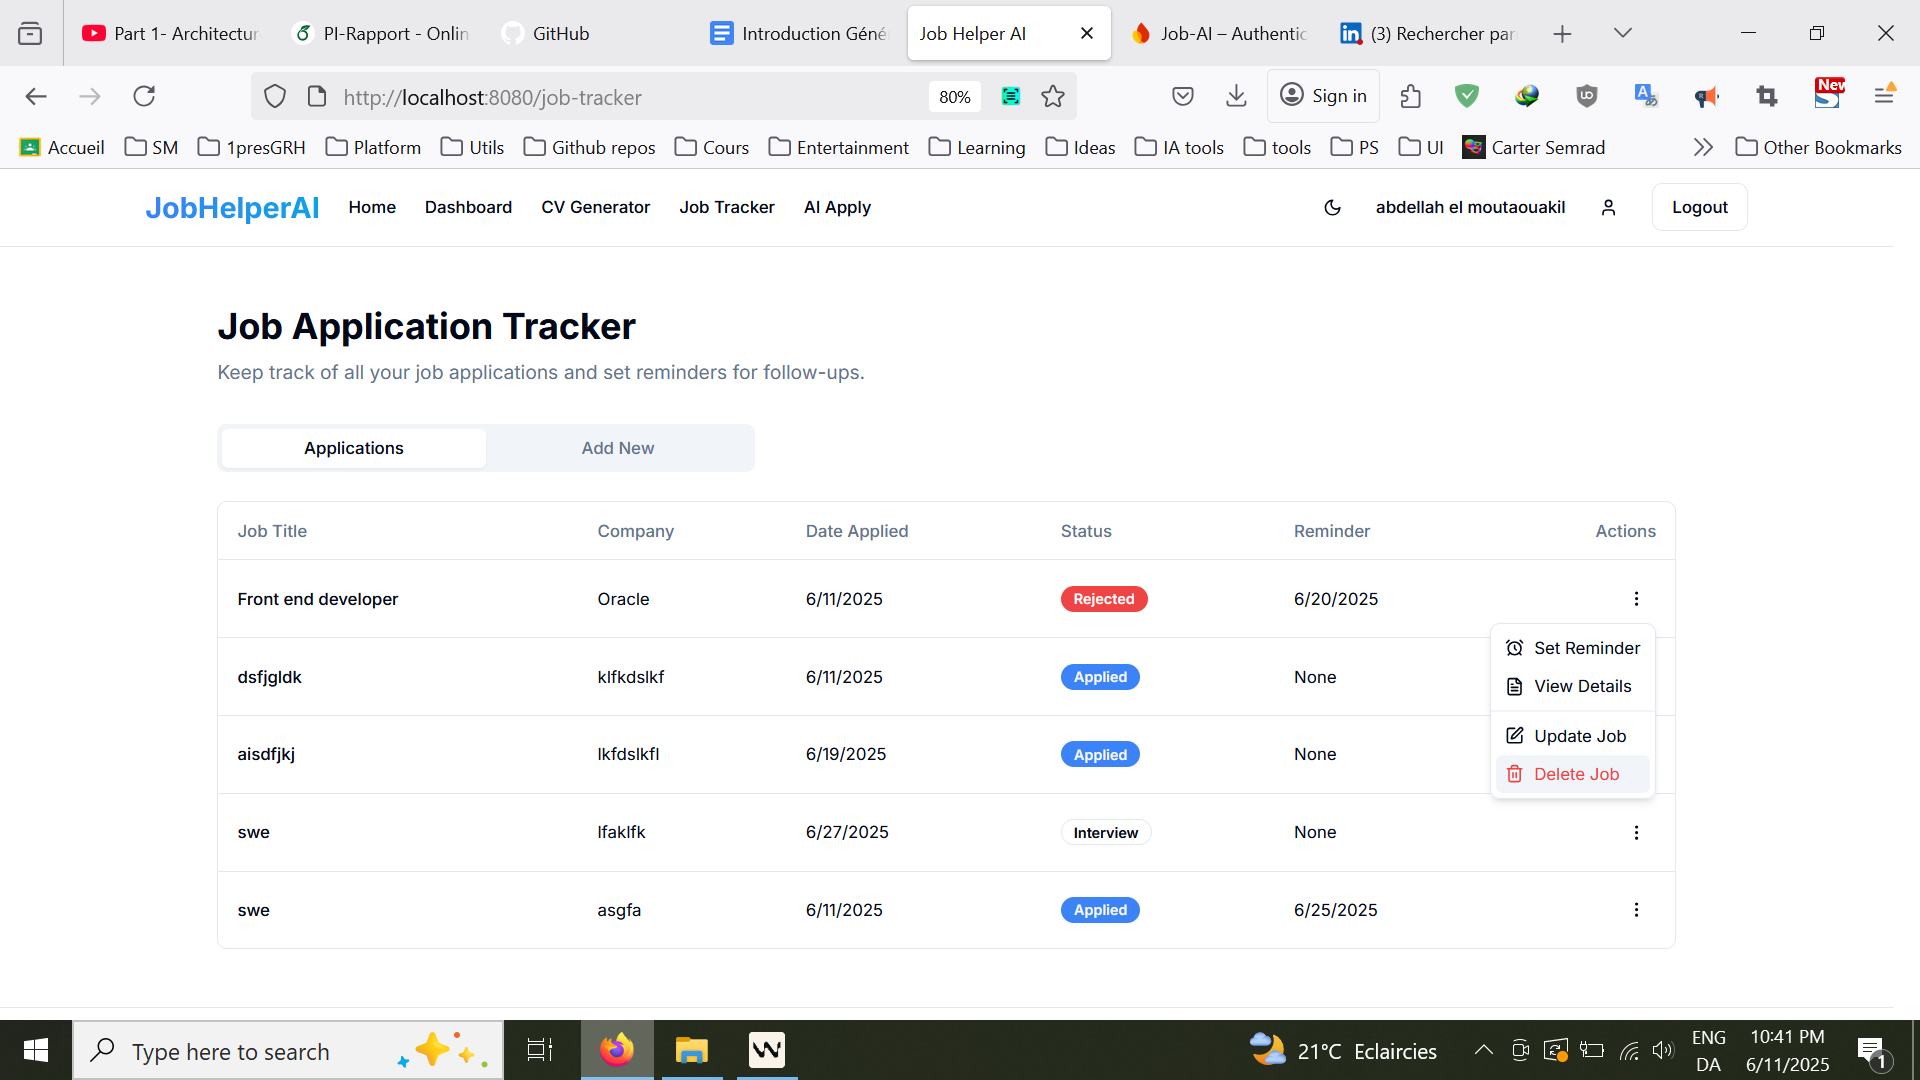
\includegraphics[width=0.8\linewidth]{screens/page_de_consultation_des_offres}}
    \caption{Interface de consultation des offres d'emploi}
    \label{fig:consultation_offres}
\end{figure}
\vspace{-0.6cm}
Cette interface présente un tableau récapitulatif complet des offres d'emploi enregistrées. Elle affiche les informations essentielles : titre du poste, entreprise, date de candidature, statut actuel, et rappels programmés. Les actions disponibles (définir un rappel, modifier, supprimer) sont accessibles directement depuis cette vue, facilitant la gestion centralisée des candidatures.

\subsubsection{Détails d'une Offre}
\vspace{-0.6cm}
\begin{figure}[H]
    \centering
      \setlength{\fboxrule}{0.2pt} % Épaisseur de la bordure
    \setlength{\fboxsep}{0pt} % Espace entre image et bordure
    \fbox{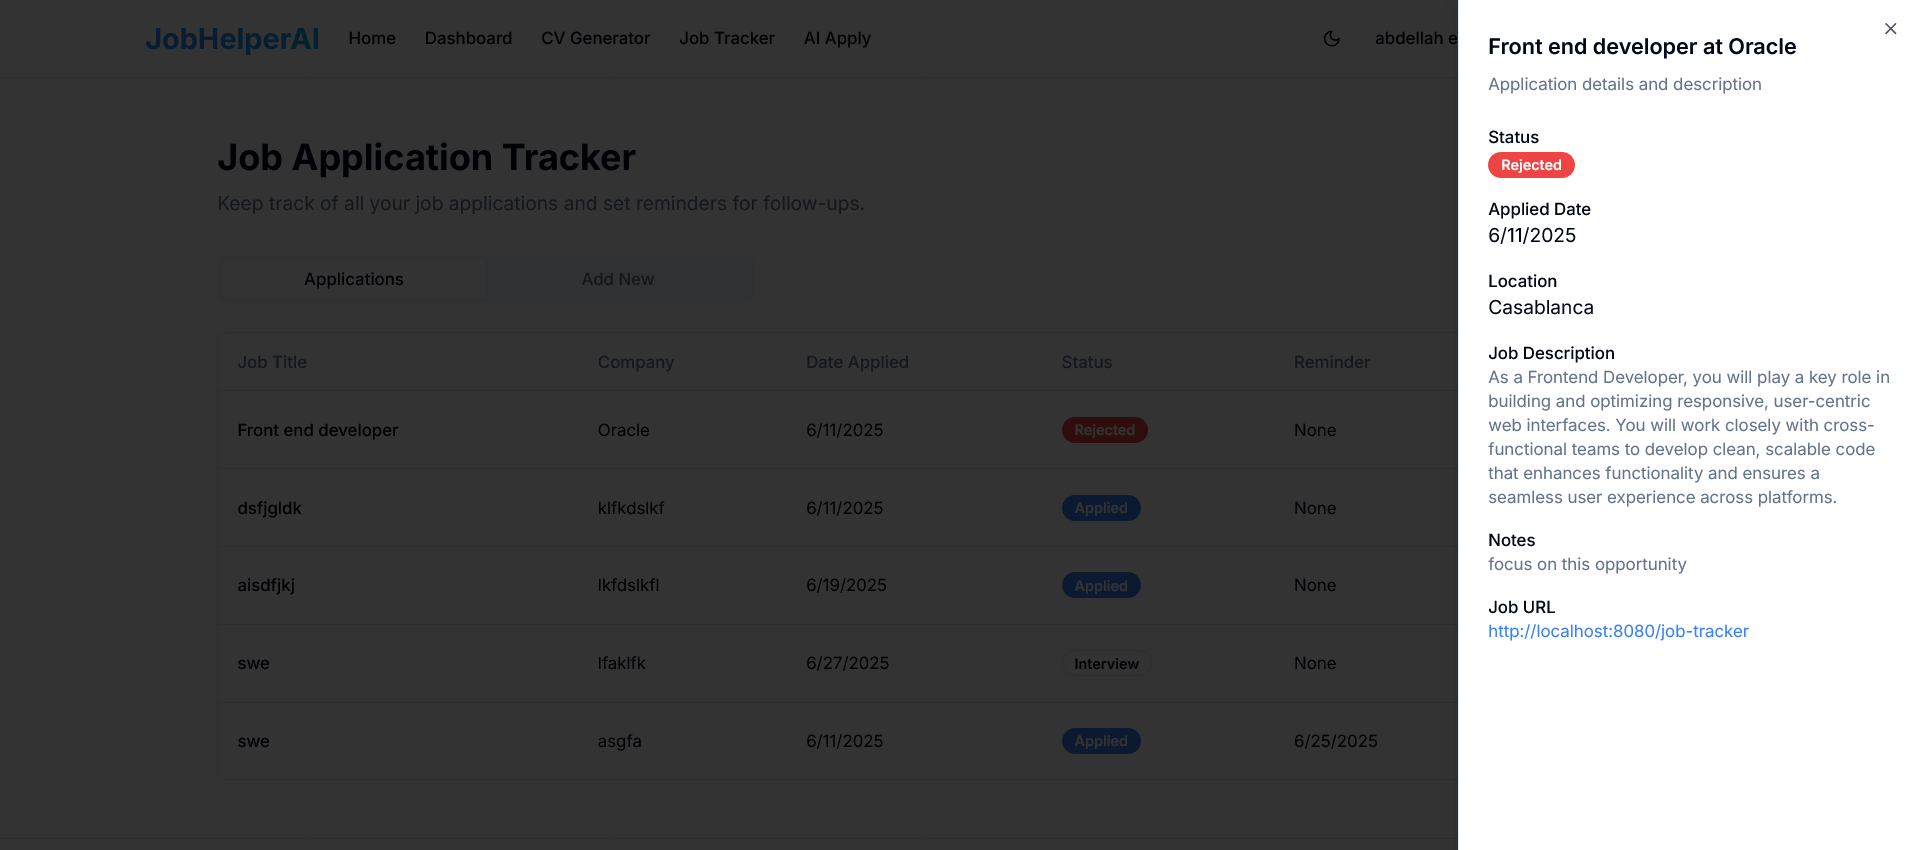
\includegraphics[width=0.8\linewidth]{screens/Consultations_de_desc_de_l_offre.png}}
    \caption{Interface de consultation détaillée d'une offre}
    \label{fig:detail_offre}
\end{figure}

La page de détails d'une offre fournit une vue approfondie d'une candidature spécifique. Elle présente la description complète du poste, les exigences de l'employeur, l'historique des interactions, et les documents associés. Cette interface permet un suivi précis de chaque opportunité professionnelle.
\vspace{-0.5cm}
\subsubsection{Ajout Manuel d'Offres}
\vspace{-0.5cm}
\begin{figure}[H]
    \centering
    \setlength{\fboxrule}{0.2pt} % Épaisseur de la bordure
    \setlength{\fboxsep}{0pt} % Espace entre image et bordure
    \fbox{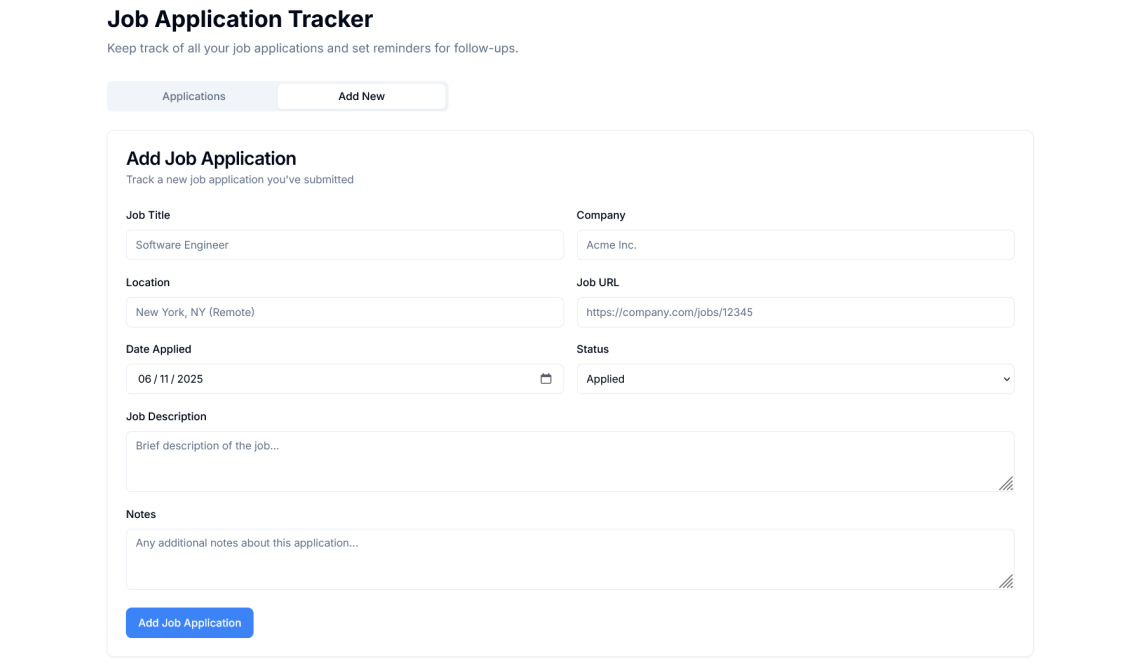
\includegraphics[width=0.8\linewidth]{screens/l_ajout_des_offres_manuellement.png}}
    \caption{Interface d'ajout manuel d'offres d'emploi}
    \label{fig:ajout_offre}
\end{figure}
\vspace{-0.5cm}
Cette interface permet aux utilisateurs d'enregistrer manuellement de nouvelles offres d'emploi dans leur système de suivi. Le formulaire structuré collecte toutes les informations pertinentes : détails du poste, informations sur l'entreprise, exigences, et notes personnelles. 
\subsection{Gestion du Profil Utilisateur}
\vspace{-0.5cm}
\begin{figure}[H]
    \centering
    \begin{minipage}{0.48\textwidth}
        \centering
        \fbox{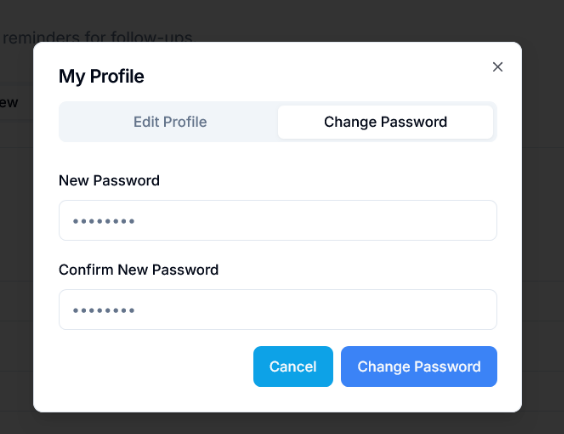
\includegraphics[width=0.95\linewidth]{screens/modif_mot_de_passe.png}}
        \vspace{0.2cm}
        \caption{Modification mot de passe}
        \label{fig:modif_mdp}
    \end{minipage}
    \hfill
    \begin{minipage}{0.48\textwidth}
        \centering
        \fbox{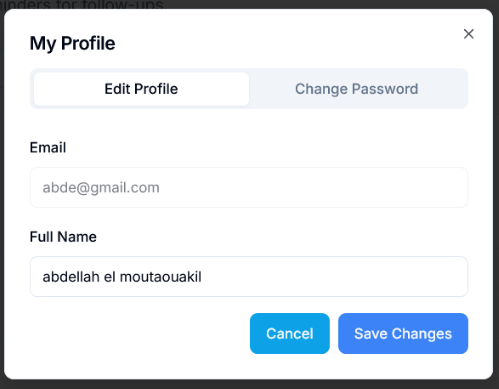
\includegraphics[width=0.95\linewidth]{screens/modif_info.png}}
        \vspace{0.2cm}
        \caption{Modification informations}
        \label{fig:modif_info}
    \end{minipage}
\end{figure}
\vspace{-0.5cm}
\textbf{Informations personnelles} : Interface claire pour mise à jour des données personnelles avec validation avant enregistrement via boutons "Annuler/Sauvegarder".\\

\textbf{Mot de passe} : Fonction sécurisée exigeant le mot de passe actuel et confirmation du nouveau, permettant une gestion autonome des accès.

\subsection{Extension Chrome JobAI}

L'extension Chrome de JobAI révolutionne la façon dont les utilisateurs collectent et gèrent les offres d'emploi en ligne. Cette solution innovante permet de capturer et sauvegarder automatiquement des opportunités professionnelles tout en naviguant naturellement sur des sites spécialisés comme LinkedIn, Welcome to the Jungle ou Indeed, sans interrompre le flux de navigation habituel.

\subsubsection{Architecture et Fonctionnement}

L'extension intègre un système RAG (Retrieval-Augmented Generation) sophistiqué qui analyse et extrait intelligemment les informations pertinentes des offres d'emploi sélectionnées. Cette technologie permet une compréhension contextuelle du contenu et une extraction précise des données structurées essentielles.

\subsubsection{Interface d'Authentification}

\begin{figure}[H]
    \centering
    \begin{subfigure}[b]{0.45\textwidth}
        \centering
        \setlength{\fboxrule}{0.2pt} % Épaisseur de la bordure
        \setlength{\fboxsep}{0pt} % Espace entre image et bordure
        \fbox{
\includegraphics[width=0.9\linewidth]{screens/extension.png}}
        \caption{Interface principale de l'extension}
        \label{fig:extension_main}
    \end{subfigure}
    \hfill
    \begin{subfigure}[b]{0.45\textwidth}
        \centering
        \setlength{\fboxrule}{0.2pt} % Épaisseur de la bordure
        \setlength{\fboxsep}{0pt} % Espace entre image et bordure
        \fbox{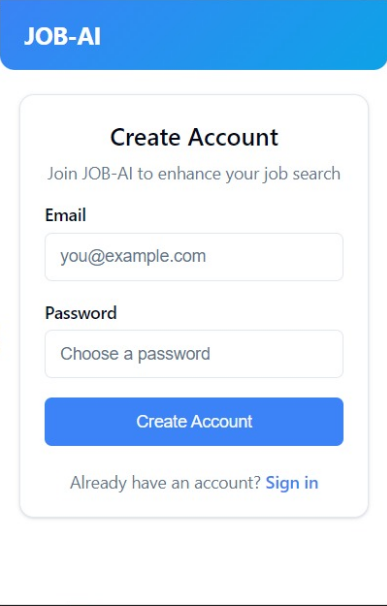
\includegraphics[width=0.94\linewidth]{screens/exntention-Login.png}}
        \caption{Interface de connexion de l'extension}
        \label{fig:extension_login}
    \end{subfigure}
    \caption{Interfaces d'accueil et d'authentification de l'extension Chrome}
    \label{fig:extension_auth}
\end{figure}

L'extension propose une interface d'authentification sécurisée qui permet aux utilisateurs de se connecter directement depuis leur navigateur.

\subsubsection{Détection et Capture d'Offres}

\begin{figure}[H]
    \centering
    \begin{subfigure}[b]{0.48\textwidth}
        \centering
        \setlength{\fboxrule}{0.2pt} % Épaisseur de la bordure
        \setlength{\fboxsep}{0pt} % Espace entre image et bordure
        \fbox{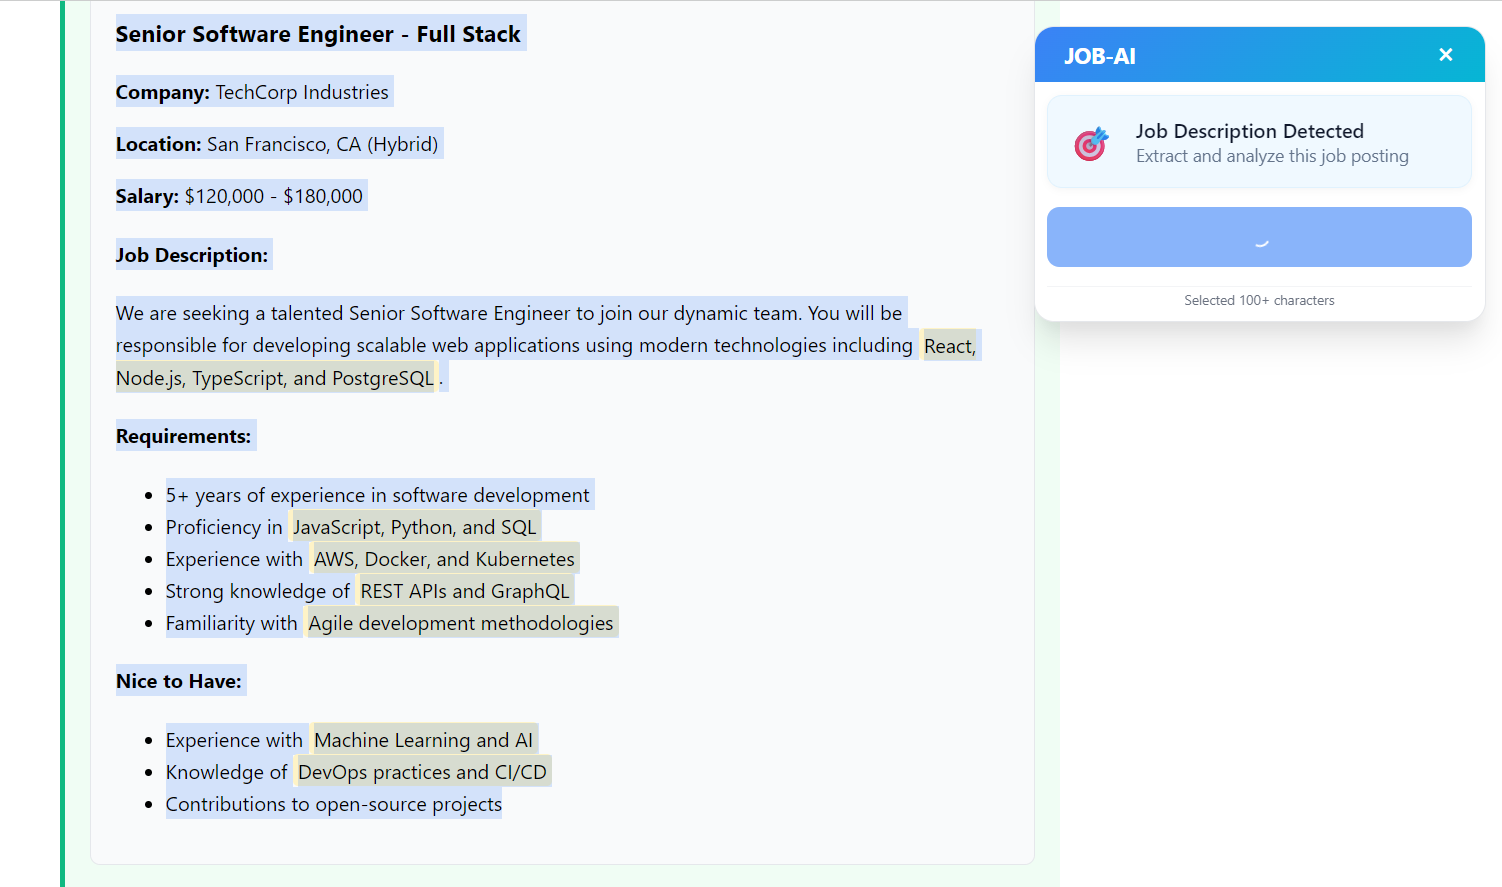
\includegraphics[width=1\linewidth]{screens/Detection-Offre.png}}
        \caption{Détection automatique d'une offre}
        \label{fig:detection_offre}
    \end{subfigure}
    \hfill
    \begin{subfigure}[b]{0.48\textwidth}
        \centering
        \setlength{\fboxrule}{0.2pt} % Épaisseur de la bordure
        \setlength{\fboxsep}{0pt} % Espace entre image et bordure
        \fbox{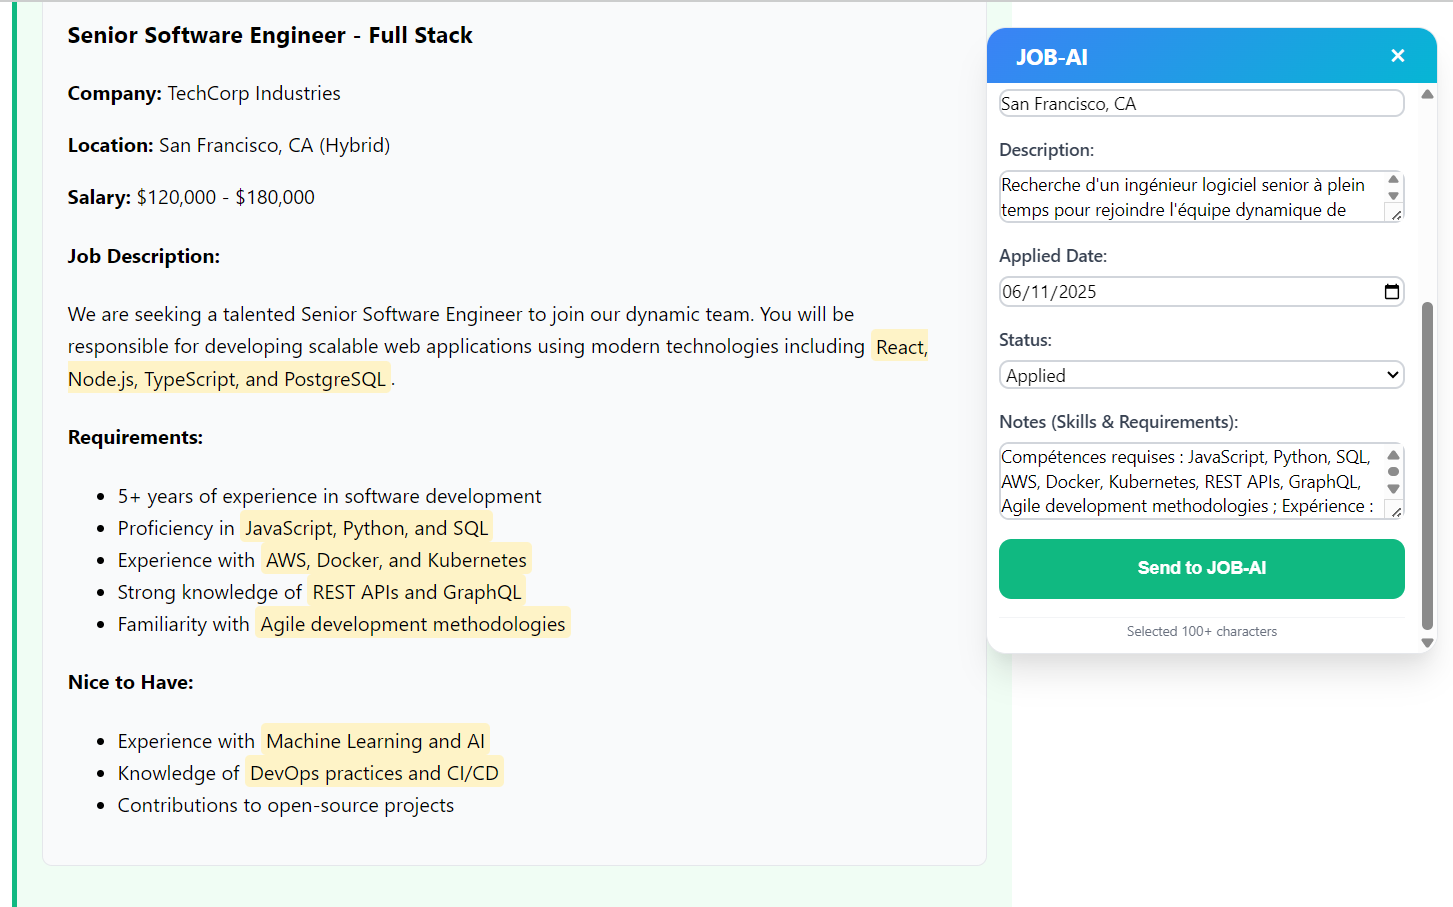
\includegraphics[width=1\linewidth]{screens/widget-Offre-details-extracted-with-add-button-to-job-liste.png}}
        \caption{Widget d'extraction des détails}
        \label{fig:widget_extraction}
    \end{subfigure}
    \caption{Processus de détection et d'extraction des offres d'emploi}
    \label{fig:detection_extraction}
\end{figure}

Le processus de capture s'active simplement par la sélection de texte d'une offre sur une page web. Un widget contextuel intelligent apparaît instantanément, permettant à l'utilisateur de visualiser les informations extraites et de les modifier si nécessaire avant sauvegarde.

\subsubsection{Processus d'Extraction Intelligent}

Le système RAG intégré à l'extension analyse le texte sélectionné selon plusieurs étapes :

\begin{enumerate}
    \item \textbf{Analyse contextuelle} : Identification automatique du type de contenu et de sa structure
    \item \textbf{Extraction des entités} : Recognition des éléments clés (titre du poste, entreprise, localisation, etc.)
    \item \textbf{Structuration des données} : Organisation des informations selon un schéma prédéfini
    \item \textbf{Validation et présentation} : Affichage des données extraites dans un formulaire éditable
\end{enumerate}

\subsubsection{Fonctionnalités Avancées}

\paragraph{Édition en Temps Réel}
L'interface de widget permet aux utilisateurs de modifier directement les informations extraites avant leur sauvegarde. Cette fonctionnalité garantit la précision des données collectées et permet d'ajouter des notes personnelles ou des détails complémentaires.

\paragraph{Synchronisation Automatique}
Une fois validées, les offres capturées sont automatiquement synchronisées avec la plateforme JobAI principale. Elles apparaissent instantanément dans l'interface de gestion des candidatures, prêtes pour analyse et traitement par les autres modules de l'écosystème.

\subsection{Génération de Documents Professionnels}

\subsubsection{Ajout du CV}

\begin{figure}[H]
    \centering
    \begin{subfigure}[c]{0.45\linewidth}
        \centering
        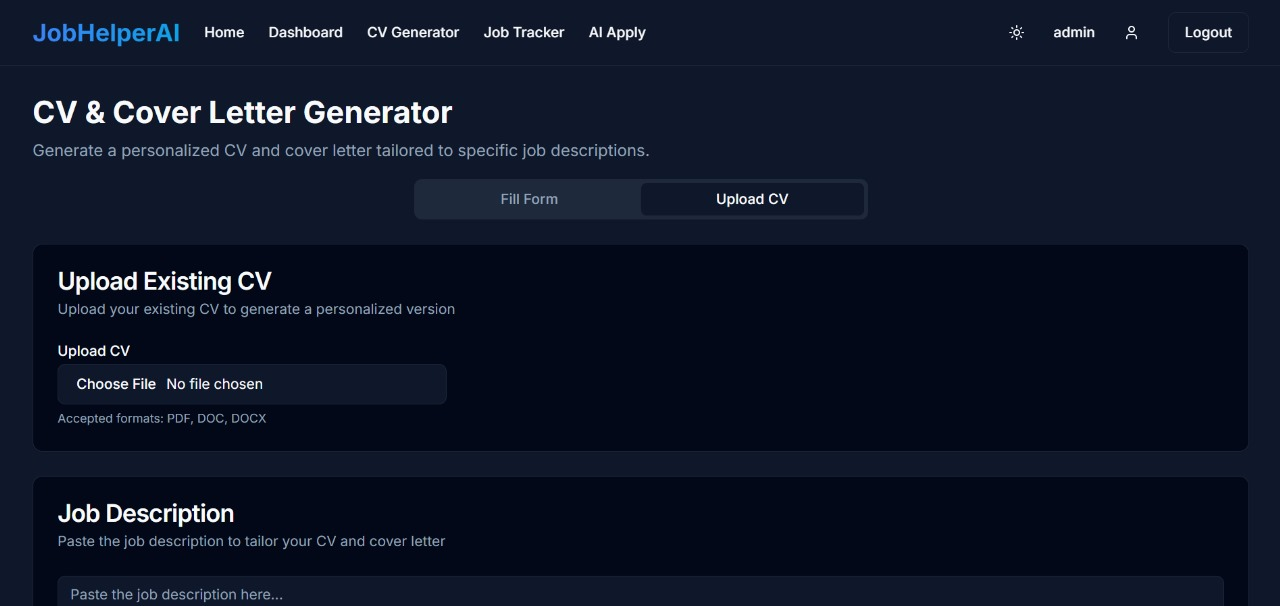
\includegraphics[width=\linewidth]{screens/cv-auto.jpeg}
        \caption{Formulaire de génération automatique.}
        \label{fig:cv-auto}
    \end{subfigure}
    \hfill
    \begin{subfigure}[c]{0.45\linewidth}
        \centering
        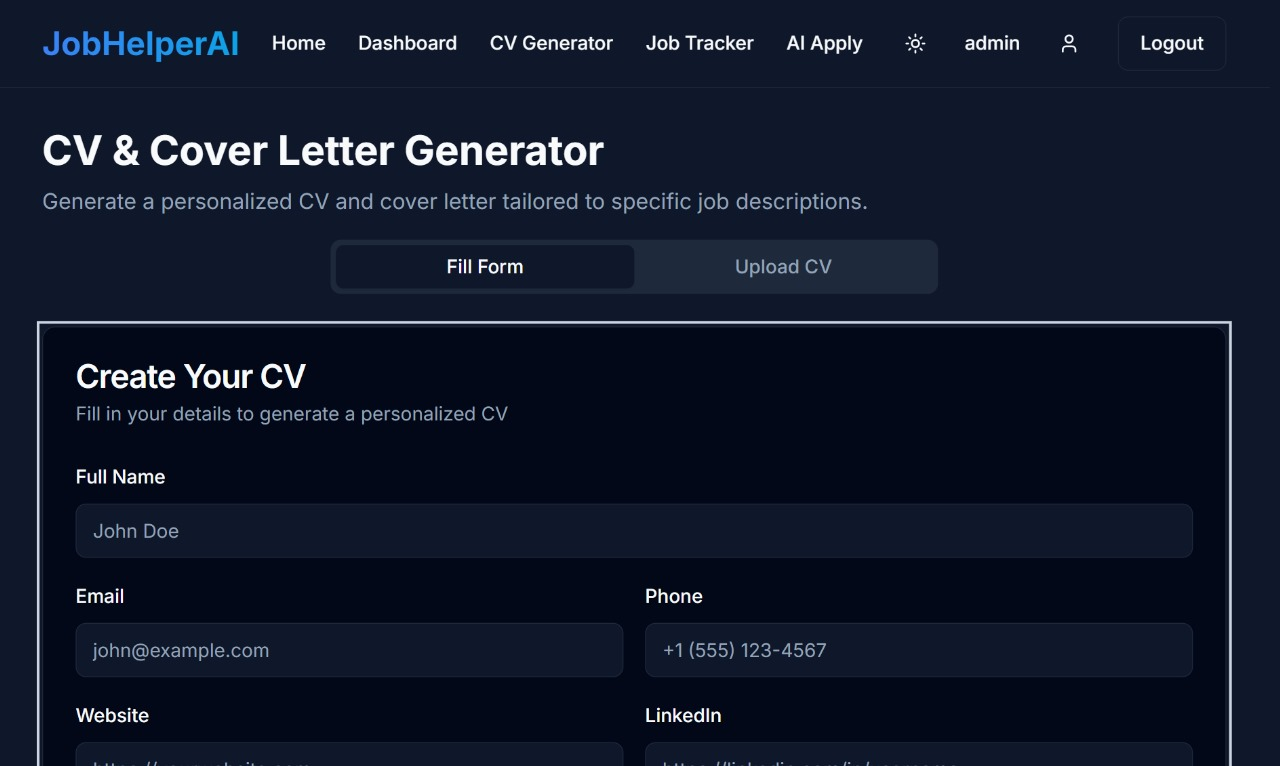
\includegraphics[width=\linewidth]{screens/cv-Manuelle.jpeg}
        \caption{Remplissage manuel des informations.}
        \label{fig:cv-manuelle}
    \end{subfigure}
    \caption{Interface de génération de CV exploitant l’intelligence artificielle.}
    \label{fig:generation-cv-global}
\end{figure}

L’interface de génération de CV permet à l’utilisateur soit de remplir un formulaire structuré avec ses informations, soit de téléverser un CV existant. Dans ce dernier cas, un modèle d’intelligence artificielle (LLM) analyse automatiquement le document et remplit le formulaire à sa place. L’utilisateur peut ensuite visualiser un aperçu et générer un CV optimisé selon les standards professionnels actuels.

\begin{figure}[H]
    \centering
    \setlength{\fboxrule}{0.2pt} % Épaisseur de la bordure
        \setlength{\fboxsep}{0pt} % Espace entre image et bordure
        \fbox{
\includegraphics[width=1\linewidth]{screens/Add-offre.png}}
    \caption{Interface d’ajout d’une offre d’emploi.}
    \label{fig:add-offre}
\end{figure}

Cette interface permet à l’utilisateur d’ajouter manuellement une offre d’emploi. Les informations saisies sont ensuite utilisées par le système pour adapter automatiquement le CV et la lettre de motivation en fonction des exigences du poste. Cela garantit une meilleure adéquation entre le profil du candidat et les attentes des recruteurs.\\

\subsection{Analyse de Compatibilité}
\begin{figure}[H]
    \centering
    \setlength{\fboxrule}{0.2pt} % Épaisseur de la bordure
    \setlength{\fboxsep}{0pt} % Espace entre image et bordure
    \fbox{
\includegraphics[width=0.8\linewidth]{screens/Cv-Feedback.png}}
    \caption{Interface d'analyse de compatibilité profil-offre}
    \label{fig:analyse_compatibilite}
\end{figure}

L'interface d'analyse de compatibilité utilise l'intelligence artificielle pour évaluer l'adéquation entre le profil du candidat et une offre d'emploi. Elle présente un score de compatibilité détaillé, identifie les points forts et les lacunes, et propose des recommandations d'amélioration. Cette fonctionnalité aide les utilisateurs à prioriser leurs candidatures et à optimiser leur profil professionnel.

\begin{figure}[H]
    \centering
    \setlength{\fboxrule}{0.2pt} % Épaisseur de la bordure
    \setlength{\fboxsep}{0pt} % Espace entre image et bordure
    \fbox{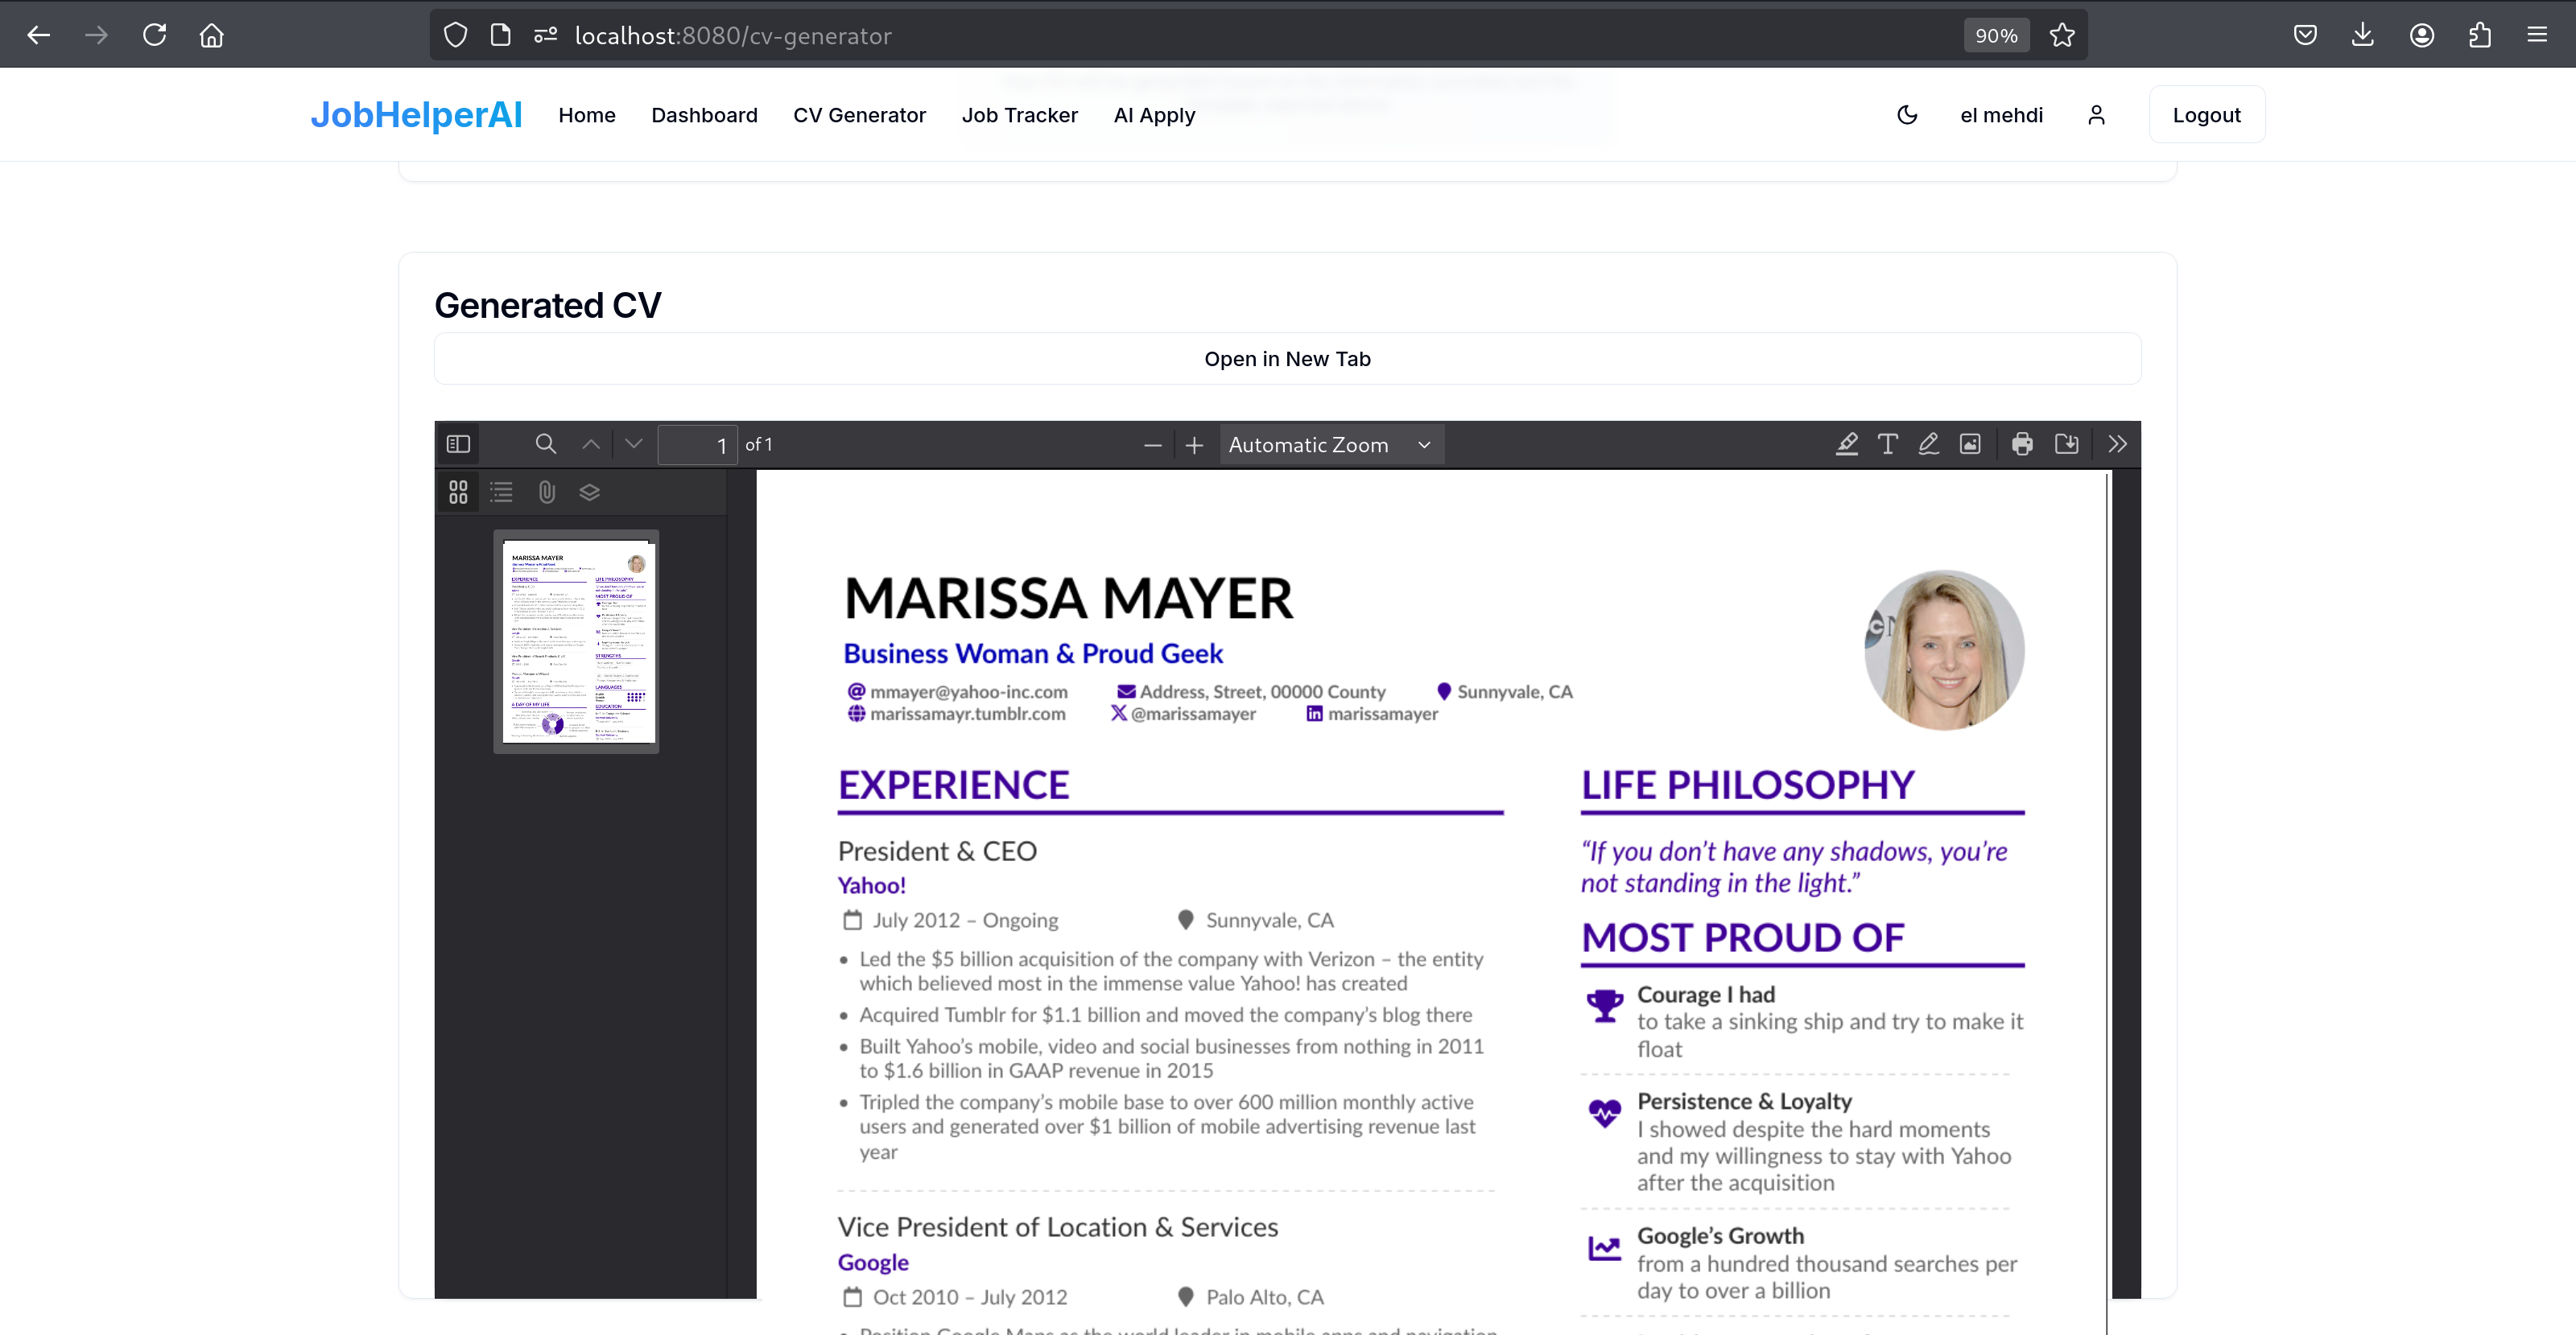
\includegraphics[width=1\linewidth]{screens/cv-Preview.jpg}}
    \caption{Aperçu du CV généré par l’IA.}
    \label{fig:cv-preview}
\end{figure}

Le modèle d’intelligence artificielle propose une version optimisée du CV selon les bonnes pratiques actuelles. Il adapte la mise en page, reformule certaines phrases et met en avant les compétences pertinentes en fonction du poste ciblé.



\subsubsection{Génération de Lettres de Motivation}
\begin{figure}[H]
    \centering
    
\includegraphics[width=0.8\linewidth]{screens/Cover-Letter.png}
    \caption{Lettre de motivation}
    \label{fig:lettre_motivation}
\end{figure}
Cette interface permet la création automatisée de lettres de motivation personnalisées. En combinant les informations du profil utilisateur avec les détails d'une offre d'emploi spécifique, le système génère une lettre adaptée au poste et à l'entreprise cible. L'utilisateur peut prévisualiser, modifier et télécharger le document final.




\subsection{Cohérence et Ergonomie}

L'ensemble des interfaces de JobAI respecte une charte graphique cohérente, privilégiant la lisibilité et l'efficacité. La navigation intuitive, les codes couleur standardisés, et les icônes expressives facilitent l'appropriation de l'outil par les utilisateurs. Cette approche design garantit une expérience utilisateur fluide et professionnelle, adaptée aux exigences de la recherche d'emploi moderne.

\section*{Conclusion}

L’ensemble des interfaces proposées dans JobAI illustre la volonté de fournir un outil complet, ergonomique et intelligent pour accompagner l’utilisateur tout au long de son parcours de recherche d’emploi. Que ce soit via le tableau de bord synthétique, la gestion fine des offres, l’extension Chrome innovante ou les fonctionnalités avancées de génération et d’analyse de CV, chaque composant a été pensé pour maximiser l’efficacité, la personnalisation et la simplicité d’usage.

Grâce à l’intégration de technologies d’intelligence artificielle telles que le système RAG pour l’extraction des offres et les modèles LLM pour l’optimisation des documents professionnels, JobAI se positionne comme une solution moderne et adaptée aux besoins actuels des candidats, facilitant la gestion proactive de leurs candidatures et améliorant leurs chances de succès.
	% \include{pages/08-conclusion-perspectives}
	% \include{pages/09-annexes}
	
	%-------------------- End of Document ---------------------%
\end{document}
